 \documentclass[lettersize,journal]{IEEEtran}
\usepackage{amsmath,amssymb,amsfonts}
\usepackage{algorithmic}
\usepackage{algorithm}
\usepackage{array}
\usepackage[caption=false,font=footnotesize,labelfont=rm,textfont=rm]{subfig}
\usepackage{textcomp}
\usepackage{stfloats}
\usepackage{url}
\usepackage{verbatim}
\usepackage{graphicx}
\usepackage{cite}
\usepackage{booktabs}
\usepackage{multirow}
\usepackage{color}
\usepackage{xcolor}
\usepackage{soul} 
\usepackage{tcolorbox}
\sethlcolor{red}
\soulregister{\cite}7 % 注册\cite命令
\soulregister{\citep}7 % 注册\citep命令
\soulregister{\citet}7 % 注册\citet命令
\soulregister{\ref}7 % 注册\ref命令
\soulregister{\pageref}7 % 注册\pageref命令
\usepackage[table]{xcolor}


\hyphenation{op-tical net-works semi-conduc-tor IEEE-Xplore}
% updated with editorial comments 8/9/2021

\begin{document}

\title{WaveLoop: Wavelet-Guided Temporal-Frequency Modeling for Video Crowd Counting}

\author{Junyu Sun, Miaogen Ling, Wei Fang and Xin Geng,~\IEEEmembership{Senior Member,~IEEE}
        % <-this % stops a space
% \thanks{This paper was produced by the IEEE Publication Technology Group. They are in Piscataway, NJ.}% <-this % stops a space
\thanks{Manuscript received **; revised **. This research is supported by the Jiangsu Science Foundation (BG2024036, BK20243012), the National Science Foundation of China (62202235, 62125602, U24A20324, 92464301), the New Cornerstone Science Foundation through the XPLORER PRIZE, and the Fundamental Research Funds for the Central Universities (2242025K30024). \textit{(Corresponding author: Xin Geng.)}}
\thanks{Miaogen Ling is with the School of Computer Science, Nanjing University of Information Science and Technology, Nanjing 210044, China, and also with the Provincial Key Laboratory for Computer Information Processing Technology, Soochow University, Suzhou 215006, China (e-mail: mgling@nuist.edu.cn).}
\thanks{Junyu Sun and Wei Fang are with the School of Computer Science, Nanjing University of Information Science and Technology, Nanjing 210044, China (e-mail: 202412492179@nuist.edu.cn; fangwei@nuist.edu.cn).}
\thanks{Xin Geng is with the School of Computer Science and Engineering, Southeast University, Nanjing 211189, China (e-mail: xgeng@seu.edu.cn).}
\thanks{Copyright © 2026 IEEE. Personal use of this material is permitted. However, permission to use this material for any other purposes must be obtained from the IEEE by sending an email to pubs-permissions@ieee.org.}
}

% The paper headers
\markboth{IEEE Transactions on Multimedia}%
{Shell \MakeLowercase{\textit{et al.}}: A Sample Article Using IEEEtran.cls for IEEE Journals}

% \IEEEpubid{0000--0000/00\$00.00~\copyright~2021 IEEE}
% Remember, if you use this you must call \IEEEpubidadjcol in the second
% column for its text to clear the IEEEpubid mark.

\maketitle

\begin{abstract}
Video crowd counting benefits from temporal cues in consecutive frames, but existing methods typically entangle temporal dynamics within multi-frame features or rely on explicit motion representations that mainly describe abrupt inter-frame changes. Consequently, temporally shared crowd structure and rapid variations are not jointly exploited, while the complementary spatial- and frequency-domain representations remain difficult to coordinate. We propose WaveLoop, a wavelet-guided temporal-frequency network for accurate video crowd counting. WaveLoop first applies spatial discrete wavelet transform to the current frame and introduces Scale-Aligned Frequency Fusion to balance the magnitude distributions of low- and high-frequency sub-bands, producing a detail-preserving frequency representation. It further decomposes two adjacent frames along the temporal dimension into a low-frequency component that preserves temporally shared context and a high-frequency component that captures rapid inter-frame variations. A Temporal Frequency Reconfiguration module uses the former for channel-wise modulation and the latter for motion-sensitive deformable aggregation, thereby injecting complementary temporal cues into the current-frame frequency features. To coordinate spatial and frequency representations, Density-Guided Frequency Attention adapts cross-domain interaction using density-aware spatial priors, while Dual-Domain Similarity Enhancement reinforces reliable responses shared by temporal-frequency and spatial-frequency features without discarding their complementary information. A supervised density-variation objective further regularizes density changes across adjacent predictions. Extensive experiments on five benchmark datasets demonstrate the effectiveness of WaveLoop. In particular, it improves MAE and RMSE by 8.5\% and 9.9\%, respectively, over the strongest competing method on the Classroom dataset.
\end{abstract}



\begin{IEEEkeywords}
Video crowd counting, temporal-frequency modeling, discrete wavelet transform, spatial-frequency interaction, density-variation learning.
\end{IEEEkeywords}




\section{Introduction}
\label{Intro}
\IEEEPARstart{V}{ideo} crowd counting aims to estimate a density map for each frame while exploiting the temporal continuity of crowd distributions. Compared with single-image counting, consecutive frames provide complementary observations that can alleviate appearance ambiguity caused by severe occlusion, scale variation, and motion blur. However, effectively extracting temporal information without introducing unstable cross-frame predictions remains challenging.

Existing video crowd counting methods can be broadly divided into spatiotemporal modeling and motion-guided approaches. Spatiotemporal modeling methods \cite{xiong2017spatiotemporal,zou2019enhanced,ma2021spatiotemporal,dong2022clrnet,cai2022global,wu2022spatial,ling2025dual,ling2026dual,ling2026cascaded} aggregate features from multiple consecutive frames through 3D convolutions, recurrent structures, or attention mechanisms. Although effective, they commonly represent different temporal patterns within entangled multi-frame features and may introduce additional computation and memory consumption as the temporal window grows. Motion-guided methods instead employ optical flow \cite{ranjan2017optical,hossain2020video,hou2023frame,cao2024efficient} or frame differences \cite{ling2023motional} to highlight dynamic regions. Such explicit motion cues are useful for capturing rapid inter-frame changes, but they reduce temporal information mainly to motion-sensitive residuals and may insufficiently preserve the stable crowd structure shared by adjacent frames.

These limitations raise three closely related questions. First, how can temporally shared content and rapid variations be represented in a unified manner? Crowd videos contain both relatively stable density structure and motion-sensitive changes, whereas treating temporal information as either an undifferentiated multi-frame feature or a single motion residual cannot explicitly distinguish these complementary components. Second, how can temporal cues be effectively injected into the current-frame representation? Direct feature aggregation may obscure their different roles: stable temporal context is more suitable for global feature modulation, while rapid variations require spatially adaptive modeling. Third, spatial and frequency representations exhibit different statistics and semantics. In particular, spatial wavelet sub-bands have substantially different magnitudes, and subsequent spatial--frequency interaction may be dominated by one representation if they are simply added or concatenated. These issues can weaken density-sensitive features and cause unstable predictions across consecutive frames.

To address these challenges, we propose WaveLoop, a wavelet-guided temporal-frequency framework for video crowd counting. The central idea is to model temporal dynamics through frequency separation rather than relying solely on explicit motion extraction. Given two adjacent frames, a temporal discrete wavelet transform (DWT-T) decomposes them into a temporal low-frequency component and a temporal high-frequency component. The low-frequency component preserves temporally shared context between the two frames, whereas the high-frequency component characterizes rapid inter-frame variations, including motion-sensitive changes. Based on their distinct properties, we develop a Temporal Frequency Reconfiguration Module (TFRM) that injects the two components into the current-frame frequency representation through complementary operations. Specifically, the temporal low-frequency feature generates channel-wise scaling and shifting parameters to adapt the global feature response, while the temporal high-frequency feature predicts offsets and modulation masks for deformable aggregation. This design enables stable temporal context and localized dynamic changes to jointly refine the current-frame representation.

We further construct a spatial--frequency collaboration pathway to preserve density-critical structures. A spatial discrete wavelet transform (DWT-S) first decomposes the current frame into one low-frequency and three directional high-frequency sub-bands. Since these sub-bands have markedly different value ranges, the proposed Scale-Aligned Frequency Fusion (SAFF) module adaptively rescales the high-frequency representation before residual aggregation, preventing structural information or fine details from dominating the fused feature. In parallel, the original frame is encoded to provide spatial semantic features. The Density-Guided Frequency Attention (DGFA) module then uses an auxiliary density prior estimated from the spatial branch to adapt the attention temperature during spatial--frequency interaction, encouraging the model to focus on density-relevant regions. Finally, the Dual-Domain Similarity Enhancement (DSE) module measures pixel-wise consistency between the temporal-frequency and spatial-frequency representations and reinforces their reliable shared responses while retaining complementary information. The above operations are performed progressively at multiple feature scales to generate the density map of the current frame.

To reduce undesirable fluctuations between adjacent estimates, we additionally impose a temporal consistency loss on density-map variations. Rather than directly forcing two neighboring predictions to be identical, the loss aligns the predicted inter-frame density change with its ground-truth counterpart, allowing genuine crowd dynamics to be preserved while suppressing inconsistent variations. In this way, WaveLoop coordinates temporal-frequency modeling, spatially guided frequency enhancement, and prediction-level temporal regularization within a unified framework.

The main contributions are summarized as follows:
\begin{itemize}
    \item We introduce a temporal-frequency perspective for video crowd counting. By decomposing adjacent frames into temporally shared and rapidly varying components, WaveLoop explicitly models complementary temporal patterns without relying solely on an optical-flow representation or an undifferentiated multi-frame feature.

    \item We develop a structured frequency collaboration mechanism that progressively balances spatial wavelet sub-bands, injects complementary temporal cues, and incorporates density-aware spatial guidance. The resulting SAFF, TFRM, DGFA, and DSE modules form a coherent pathway from frequency construction to cross-domain enhancement, rather than performing independent feature aggregation.

    \item We introduce prediction-level temporal variation supervision to regularize cross-frame density changes. Extensive experiments on five benchmark datasets demonstrate the effectiveness of the proposed framework, including MAE and RMSE improvements of 8.5\% and 9.9\%, respectively, over the strongest competing method on the Classroom dataset.
\end{itemize}

\begin{figure}[h]
 \centering  
 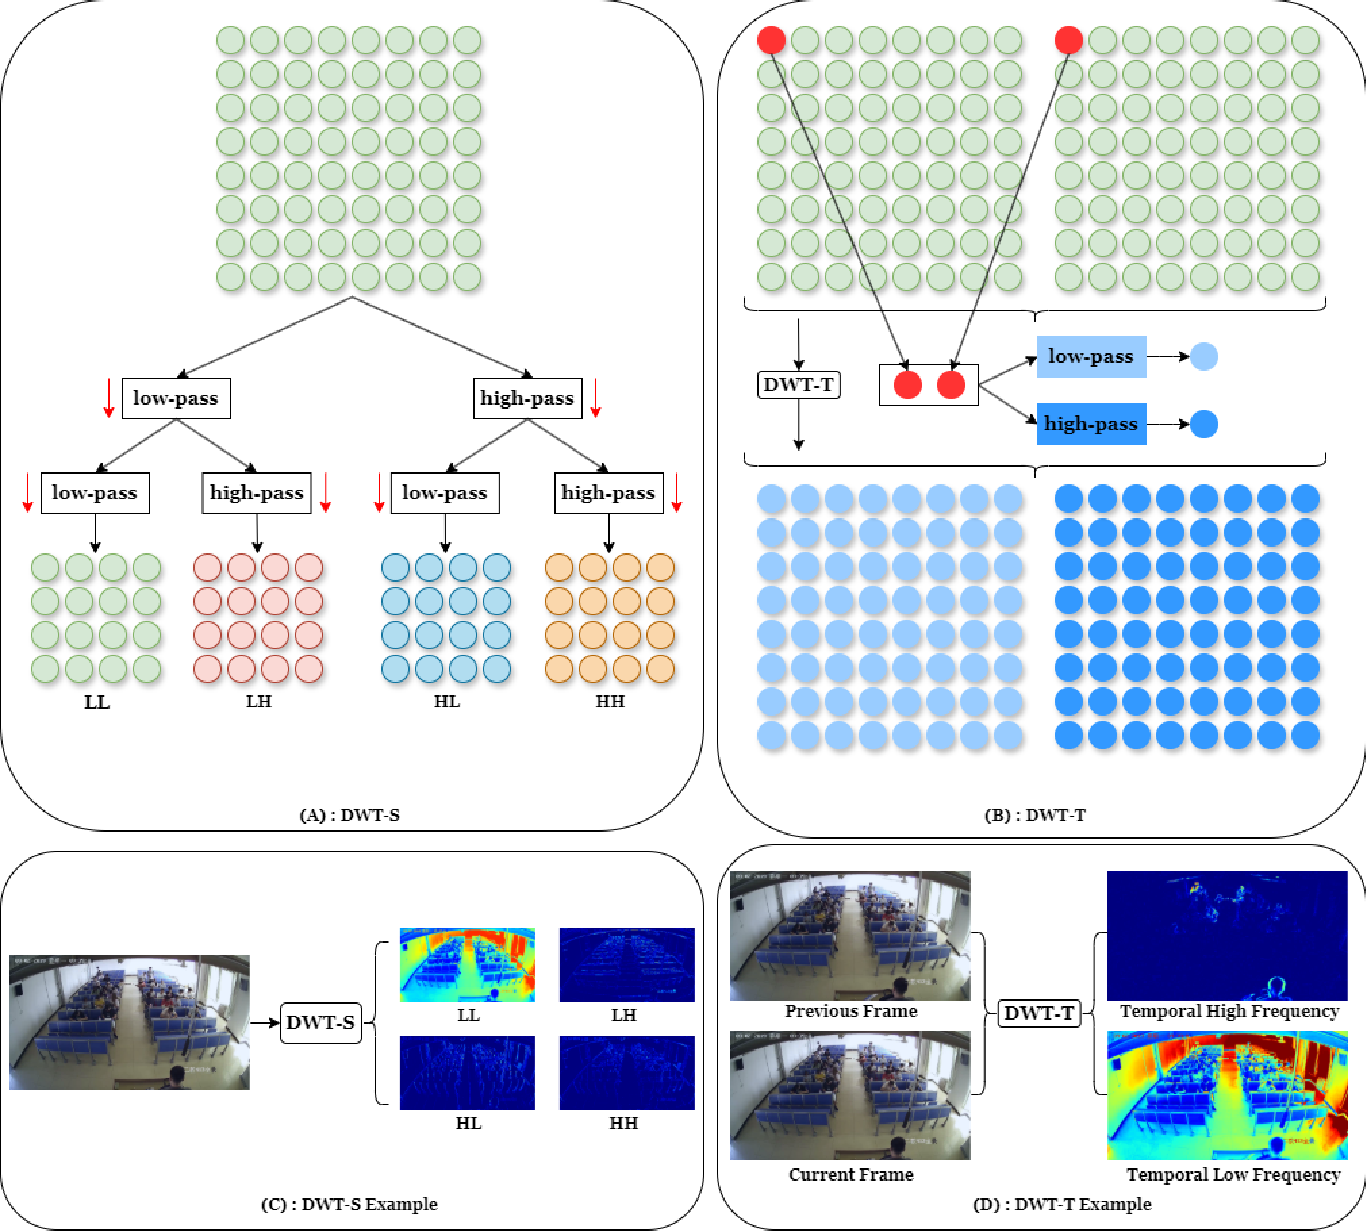
\includegraphics[width=0.47\textwidth]{Example.pdf}
    \caption{Illustration of spatial and temporal discrete wavelet transforms. (A) DWT-S decomposes a frame into one low-frequency sub-band ($LL$) and three directional high-frequency sub-bands ($LH$, $HL$, and $HH$). (B) DWT-T decomposes two adjacent frames along the temporal dimension into low- and high-frequency components. (C) Visualization of the spatial wavelet sub-bands. (D) Visualization of the temporal low- and high-frequency components.}
\label{fig:1}
\vspace{-0.5em}
\end{figure}

\section{Related Work}

\subsection{Image-Based Crowd Counting}
Image-based crowd counting primarily estimates crowd distributions from the spatial appearance of a single image. Density-regression methods predict a continuous density map whose integral gives the crowd count, and early studies mainly addressed large scale variations through multi-column or pyramid architectures \cite{sindagi2017generating,chen2019scale,yang2020embedding}. Subsequent methods introduced density-aware attention and Transformer-based interaction to enhance discriminative representations in congested regions \cite{jiang2020attention,lin2022boosting,lin2024gramformer}. In parallel, point-based approaches directly learn head locations or point queries, improving the joint capability of counting and localization \cite{song2021rethinking,liang2022focal,liu2023point,chen2024improving}. Although these methods provide strong spatial representations, they process individual frames independently and therefore cannot exploit the temporal continuity available in crowd videos.

\subsection{Video Crowd Counting}
Video crowd counting incorporates consecutive frames to improve density estimation under occlusion, motion blur, and appearance ambiguity. One line of research jointly models multi-frame features using recurrent units, 3D convolutions, graph reasoning, or attention mechanisms \cite{xiong2017spatiotemporal,zou2019enhanced,ma2021spatiotemporal,wu2022spatial,cai2022global,dong2022clrnet,ling2025dual,ling2026dual,ling2026cascaded}. These methods learn spatial and temporal dependencies within a unified representation, but temporally stable content and rapidly varying information are generally entangled during feature aggregation.

Another line of research explicitly introduces motion-sensitive cues. Optical-flow-based methods estimate inter-frame correspondences or align adjacent features to support temporal fusion \cite{hossain2020video,hou2023frame,cao2024efficient}, whereas frame-difference-based methods derive lightweight foreground motion priors without an additional flow estimator \cite{ling2023motional}. Frame-recurrent approaches further propagate historical information across sequential predictions to improve temporal continuity \cite{hou2023frame}. Despite their effectiveness, explicit motion representations mainly emphasize inter-frame changes, while recurrent propagation accumulates historical information without explicitly distinguishing the different roles of temporally shared structure and rapid local variations.

In contrast, WaveLoop represents adjacent-frame information through temporal-frequency decomposition. Rather than treating temporal cues as an undifferentiated multi-frame feature or a single motion residual, it separates relatively stable inter-frame context from motion-sensitive variations and uses them for complementary feature modulation. This frequency-separated formulation is further coordinated with spatial density semantics to support density estimation.

\subsection{Frequency-Domain Modeling in Images and Videos}
Frequency-domain representations provide a multi-resolution view of visual signals and have been widely used to complement spatial-domain features. Discrete wavelet transform (DWT) decomposes an image into localized low- and high-frequency sub-bands \cite{mallat1989theory}. Recent dense-prediction and restoration methods exploit such frequency components to preserve structural information and fine details during feature fusion \cite{chen2024frequency,chen2024bracketing,yang2024sffnet}. Wavelet representations have also been incorporated into Transformer architectures for gesture recognition and video inpainting \cite{garg2024gestformer,zhang2024wtvi,wu2024waveformer}. These studies mainly perform spatial-frequency decomposition within individual images or frames.

Temporal wavelet decomposition has been explored in video prediction and coding to separate slowly varying temporal content from high-frequency changes \cite{jin2020exploring,lanz2019content,meyer2023learned}. More closely related to crowd analysis, Bhowmik and Wallace \cite{bhowmik2018statistical} employ a temporal-plus-spatial wavelet transform to construct a motion saliency map and extract statistical sub-band features for crowd counting. However, this approach relies on handcrafted wavelet statistics rather than end-to-end density representation learning. Existing deep wavelet methods also largely focus on image restoration, segmentation, video prediction, or coding, and do not investigate how temporally separated frequency components can perform function-specific modulation of single-frame features under density-aware spatial guidance.

Different from these studies, WaveLoop jointly applies spatial and temporal wavelet decompositions to video crowd counting. It balances heterogeneous spatial sub-bands, injects low- and high-frequency temporal cues through complementary modulation operations, and coordinates the resulting frequency representations with density-aware spatial semantics for density-map estimation.

\section{Method}
\subsection{Architecture Overview}
\label{Waveloop}
As illustrated in Fig.~\ref{fig:2}, WaveLoop estimates the density map of the current frame by jointly exploiting its spatial-frequency representation and the temporal-frequency cues extracted from an adjacent frame pair. Given the previous and current frames, denoted by $\mathbf{I}_{t-1},\mathbf{I}_{t}\in\mathbb{R}^{B\times C_0\times H\times W}$, respectively, the network consists of three coordinated pathways: a spatial pathway, a spatial-frequency pathway, and a temporal-frequency pathway.

In the spatial pathway, the current frame $\mathbf{I}_{t}$ is encoded by a spatial encoder $\mathcal{E}_{s}$ to obtain multi-scale spatial features
\begin{equation}
\{\mathbf{S}_{3},\mathbf{S}_{4}\}
=
\mathcal{E}_{s}(\mathbf{I}_{t}),
\end{equation}
where $\mathbf{S}_{3}$ and $\mathbf{S}_{4}$ have spatial resolutions of $H/16\times W/16$ and $H/32\times W/32$, respectively. These features preserve the semantic and density-related information of the current frame and subsequently provide spatial guidance for frequency-domain enhancement.

In the spatial-frequency pathway, a spatial discrete wavelet transform (DWT-S) decomposes $\mathbf{I}_{t}$ into one low-frequency sub-band and three directional high-frequency sub-bands:
\begin{equation}
\{\mathbf{X}_{t}^{LL},\mathbf{X}_{t}^{LH},
\mathbf{X}_{t}^{HL},\mathbf{X}_{t}^{HH}\}
=
\mathcal{W}_{s}(\mathbf{I}_{t}).
\end{equation}
The proposed Scale-Aligned Frequency Fusion (SAFF) module balances the response magnitudes of the low- and high-frequency components and aggregates them into a unified input representation $\mathbf{F}_{\mathrm{in}}$. A frequency encoder $\mathcal{E}_{f}$ then extracts multi-scale frequency features:
\begin{equation}
\{\mathbf{F}_{3},\mathbf{F}_{4}\}
=
\mathcal{E}_{f}(\mathbf{F}_{\mathrm{in}}).
\end{equation}

In the temporal-frequency pathway, we perform a one-level Haar wavelet transform along the temporal dimension of the adjacent frame pair. The temporal low- and high-frequency components are computed as
\begin{equation}
\mathbf{X}_{t}^{L}
=
\frac{\mathbf{I}_{t-1}+\mathbf{I}_{t}}{\sqrt{2}},
\qquad
\mathbf{X}_{t}^{H}
=
\left|
\frac{\mathbf{I}_{t}-\mathbf{I}_{t-1}}{\sqrt{2}}
\right|,
\label{eq:dwt_t}
\end{equation}
where $\mathbf{X}_{t}^{L}$ preserves the content shared by the two adjacent frames, whereas $\mathbf{X}_{t}^{H}$ highlights the magnitude of rapid inter-frame variations. The absolute value operation suppresses sign ambiguity and retains change intensity, but does not explicitly encode motion direction. Two lightweight temporal encoders, $\mathcal{E}_{L}$ and $\mathcal{E}_{H}$, extract the corresponding multi-scale features:
\begin{equation}
\{\mathbf{T}_{3}^{L},\mathbf{T}_{4}^{L}\}
=
\mathcal{E}_{L}(\mathbf{X}_{t}^{L}),
\qquad
\{\mathbf{T}_{3}^{H},\mathbf{T}_{4}^{H}\}
=
\mathcal{E}_{H}(\mathbf{X}_{t}^{H}).
\end{equation}
The temporal features are projected when necessary to match the channel dimensions of the spatial-frequency features.

Cross-domain refinement is performed progressively from the fourth stage to the third stage. At scale $l\in\{4,3\}$, the Temporal Frequency Reconfiguration Module (TFRM) injects the complementary temporal-frequency cues $\mathbf{T}_{l}^{L}$ and $\mathbf{T}_{l}^{H}$ into $\mathbf{F}_{l}$, producing a temporal-frequency representation $\mathbf{F}_{l}^{T}$. In parallel, the Density-Guided Frequency Attention (DGFA) module uses the spatial feature $\mathbf{S}_{l}$ to enhance $\mathbf{F}_{l}$ with density-aware spatial semantics, yielding $\mathbf{F}_{l}^{S}$. The Dual-Domain Similarity Enhancement (DSE) module then reinforces spatial locations consistently activated by the two representations and fuses them into $\mathbf{F}_{l}^{C}$. The stage-4 output is projected and upsampled to provide top-down information for stage-3 refinement. Finally, the refined feature is upsampled and fed into a regression head to predict the density map of the current frame:
\begin{equation}
\hat{\mathbf{D}}_{t}
=
\mathcal{H}_{\mathrm{den}}(\mathbf{F}_{3}^{C}).
\end{equation}
During sequential evaluation, the network is applied to overlapping adjacent frame pairs. Temporal coherence between $\hat{\mathbf{D}}_{t-1}$ and $\hat{\mathbf{D}}_{t}$ is encouraged by the variation-level consistency objective introduced in Section~\ref{ls}; the preceding prediction is not treated as an input unless an explicit density-propagation branch is implemented.

\begin{figure*}[t]
  \centering  
  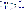
\includegraphics[width=1.0\textwidth]{fw1}
  \caption{Overview of WaveLoop. The current frame is processed by a spatial pathway and a spatial-frequency pathway, while an adjacent frame pair is decomposed along the temporal dimension to produce low- and high-frequency temporal cues. TFRM injects complementary temporal information into the current-frame frequency features, DGFA introduces density-aware spatial guidance, and DSE integrates the two enhanced representations progressively from stage 4 to stage 3. $|\cdot|$ denotes the absolute value operation, Proj denotes a $1\times1$ convolution followed by LayerNorm and GELU, and Up denotes bilinear interpolation.}
  \label{fig:2}
  \vspace{-1em}
\end{figure*}



    
\vspace{-0.5em}
\subsection{Scale-Aligned Frequency Fusion}
\label{saff}
The spatial discrete wavelet transform decomposes the current frame into a low-frequency sub-band, which mainly preserves coarse appearance and structural information, and three directional high-frequency sub-bands, which characterize horizontal, vertical, and diagonal variations. Directly aggregating these sub-bands is suboptimal because their response magnitudes differ substantially: the low-frequency component usually has a much larger energy, whereas the high-frequency components contain lower-amplitude but density-critical details. Consequently, simple addition or concatenation may lead to an imbalanced contribution of different frequency bands. We therefore introduce Scale-Aligned Frequency Fusion (SAFF), which performs channel-wise magnitude calibration before residual frequency aggregation.

Let
$\mathbf{X}_{t}^{LL},\mathbf{X}_{t}^{LH},\mathbf{X}_{t}^{HL},\mathbf{X}_{t}^{HH}
\in\mathbb{R}^{B\times C_0\times H/2\times W/2}$
denote the four sub-bands obtained from DWT-S. The three directional high-frequency sub-bands are concatenated and compressed to $C_0$ channels:
\begin{equation}
\mathbf{X}_{t}^{\mathrm{H}}
=
\operatorname{Conv}_{1\times1}
\left(
\operatorname{Concat}
\left[
\mathbf{X}_{t}^{LH},
\mathbf{X}_{t}^{HL},
\mathbf{X}_{t}^{HH}
\right]
\right).
\label{eq:high_fusion}
\end{equation}
The low- and high-frequency representations are then resized to the input resolution:
\begin{equation}
\mathbf{L}
=
\mathcal{U}(\mathbf{X}_{t}^{LL}),
\qquad
\mathbf{H}
=
\mathcal{U}(\mathbf{X}_{t}^{\mathrm{H}}),
\end{equation}
where $\mathcal{U}(\cdot)$ denotes bilinear interpolation, and
$\mathbf{L},\mathbf{H}\in\mathbb{R}^{B\times C_0\times H\times W}$.

To calibrate their response magnitudes, we compute the spatial standard deviation independently for each sample and channel. For a feature $\mathbf{X}$, it is defined as
\begin{equation}
\sigma_{h,w}(\mathbf{X})
=
\sqrt{
\frac{1}{HW}
\sum_{i=1}^{H}
\sum_{j=1}^{W}
\left(
\mathbf{X}_{:,:,i,j}
-
\mu_{h,w}(\mathbf{X})
\right)^{2}
+
\varepsilon
},
\end{equation}
where $\mu_{h,w}(\mathbf{X})$ denotes the corresponding spatial mean and $\varepsilon$ is a small constant for numerical stability. The channel-wise calibration factor is then computed as
\begin{equation}
\mathbf{R}
=
\frac{
\sigma_{h,w}(\mathbf{L})
}{
\sigma_{h,w}(\mathbf{H})+\varepsilon
},
\qquad
\mathbf{R}
\in
\mathbb{R}^{B\times C_0\times1\times1}.
\label{eq:scale}
\end{equation}
This operation rescales the high-frequency responses to a magnitude comparable to that of the low-frequency component, without assuming that the two bands follow the same semantic distribution.

Finally, the calibrated high-frequency representation is incorporated through a gated residual fusion:
\begin{equation}
\mathbf{F}_{\mathrm{in}}
=
\mathbf{L}
+
\boldsymbol{\alpha}
\odot
\mathbf{R}
\odot
\mathbf{H},
\label{eq:fusion}
\end{equation}
where
$\boldsymbol{\alpha}\in\mathbb{R}^{1\times C_0\times1\times1}$
is a learnable channel-wise parameter shared across all samples and $\odot$ denotes element-wise multiplication. The parameter $\boldsymbol{\alpha}$ allows the network to adaptively control the contribution of wavelet details after magnitude calibration. The fused representation $\mathbf{F}_{\mathrm{in}}$ is subsequently fed into the frequency encoder to obtain the multi-scale frequency features $\{\mathbf{F}_{3},\mathbf{F}_{4}\}$.

\begin{figure*}[h]
  \centering  
  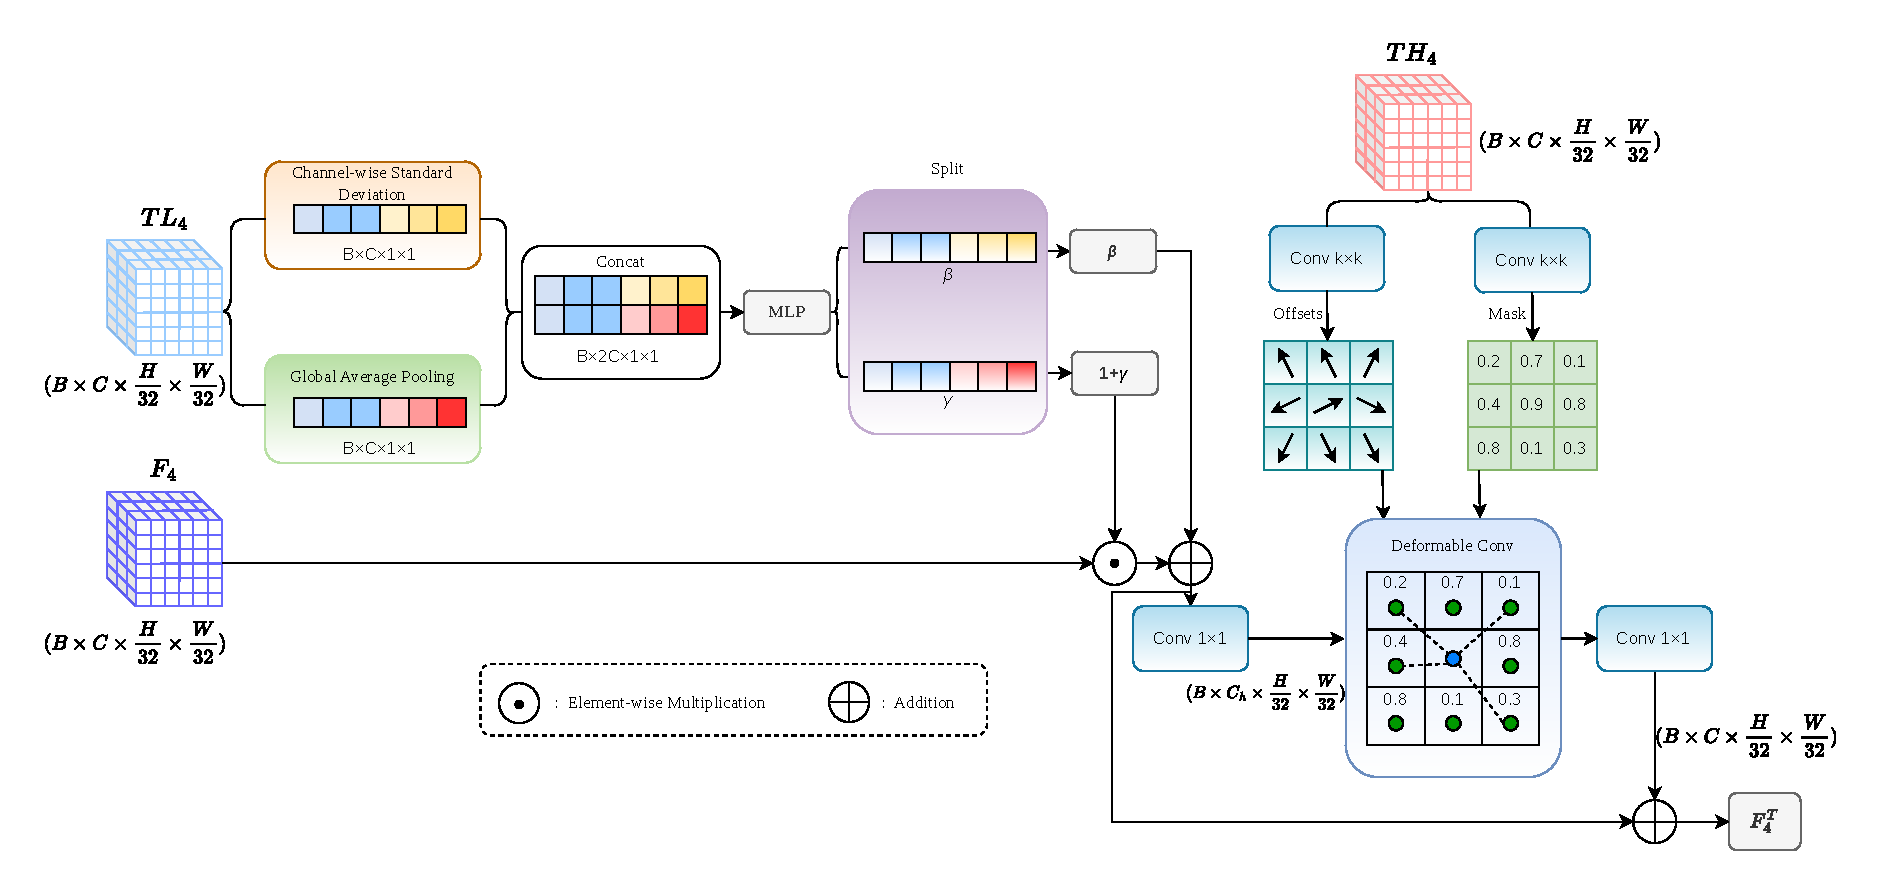
\includegraphics[width=1.0\textwidth]{tfrm.pdf}
  \caption{Temporal Frequency Reconfiguration Module (TFRM) at stage 4. The temporal low-frequency feature $\mathbf{T}_{4}^{L}$ is summarized by channel-wise mean and standard-deviation statistics to generate FiLM parameters $\boldsymbol{\gamma}_{4}$ and $\boldsymbol{\beta}_{4}$ for global feature modulation. In parallel, the temporal high-frequency feature $\mathbf{T}_{4}^{H}$ predicts deformable offsets and modulation masks to guide motion-sensitive spatial aggregation. The reconfigured feature is projected and residually added to the modulated representation, producing $\mathbf{F}_{4}^{T}$.}
  \label{fig:3}
  \vspace{-1em}
\end{figure*}

\vspace{-0.5em}
\subsection{Temporal Frequency Reconfiguration Module}
\label{TFRM}
The temporal wavelet decomposition in Eq.~\eqref{eq:dwt_t} provides two complementary cues from an adjacent frame pair. The temporal low-frequency component retains appearance and crowd structure shared across the two frames, whereas the temporal high-frequency component highlights spatial locations undergoing rapid inter-frame changes. These two cues should not be treated identically: the shared component is suitable for globally modulating the channel responses of the current-frame representation, while the rapidly varying component is more suitable for spatially adaptive aggregation. Based on this observation, we develop a Temporal Frequency Reconfiguration Module (TFRM) inspired by FiLM~\cite{perez2018film} and deformable convolution~\cite{zhu2019deformable} that combines low-frequency-conditioned feature modulation with high-frequency-guided deformable aggregation.

We describe TFRM at scale $l$, where $l\in\{3,4\}$. Given the temporal low-frequency feature
$\mathbf{T}_{l}^{L}\in\mathbb{R}^{B\times C_l\times H_l\times W_l}$,
we first compute its channel-wise mean and standard-deviation descriptors:
\begin{equation}
\mathbf{z}_{l}^{\mathrm{avg}}
=
\operatorname{GAP}(\mathbf{T}_{l}^{L}),
\end{equation}
\begin{equation}
\mathbf{z}_{l}^{\mathrm{std}}
=
\sqrt{
\operatorname{GAP}
\left[
\left(
\mathbf{T}_{l}^{L}
-
\mathbf{z}_{l}^{\mathrm{avg}}
\right)^{2}
\right]
+
\varepsilon
},
\end{equation}
where both descriptors belong to
$\mathbb{R}^{B\times C_l\times1\times1}$.
The two statistics are concatenated and transformed by a lightweight MLP to generate channel-wise scaling and shifting parameters:
\begin{equation}
[\boldsymbol{\gamma}_{l},\boldsymbol{\beta}_{l}]
=
\operatorname{MLP}_{l}
\left(
\operatorname{Concat}
\left[
\mathbf{z}_{l}^{\mathrm{avg}},
\mathbf{z}_{l}^{\mathrm{std}}
\right]
\right),
\end{equation}
where
$\boldsymbol{\gamma}_{l},\boldsymbol{\beta}_{l}
\in\mathbb{R}^{B\times C_l\times1\times1}$.
The current-frame frequency feature $\mathbf{F}_{l}$ is then modulated in a residual FiLM form:
\begin{equation}
\bar{\mathbf{F}}_{l}
=
\left(1+\boldsymbol{\gamma}_{l}\right)
\odot
\mathbf{F}_{l}
+
\boldsymbol{\beta}_{l}.
\label{eq:film}
\end{equation}
The identity term in $(1+\boldsymbol{\gamma}_{l})$ preserves the original feature path while allowing the temporally shared context to adaptively recalibrate channel responses.

We next use the temporal high-frequency feature
$\mathbf{T}_{l}^{H}$
to guide spatial reconfiguration. The modulated feature is first projected to a compact hidden representation:
\begin{equation}
\mathbf{F}_{l}^{h}
=
\mathcal{P}_{l}^{\mathrm{in}}
\left(
\bar{\mathbf{F}}_{l}
\right),
\end{equation}
where $\mathcal{P}_{l}^{\mathrm{in}}$ consists of a $1\times1$ convolution, LayerNorm, and GELU. For a deformable kernel with $K=k^{2}$ sampling points, two convolutional predictors generate the sampling offsets and modulation masks from $\mathbf{T}_{l}^{H}$:
\begin{equation}
\Delta\mathbf{P}_{l}
=
\operatorname{Conv}_{o}
\left(
\mathbf{T}_{l}^{H}
\right),
\qquad
\Delta\mathbf{P}_{l}
\in
\mathbb{R}^{B\times2K\times H_l\times W_l},
\end{equation}
\begin{equation}
\mathbf{M}_{l}
=
\sigma
\left(
\operatorname{Conv}_{m}
\left(
\mathbf{T}_{l}^{H}
\right)
\right),
\qquad
\mathbf{M}_{l}
\in
\mathbb{R}^{B\times K\times H_l\times W_l},
\end{equation}
where $\sigma(\cdot)$ is the sigmoid function. If multiple deformable groups are used, the channel dimensions above are multiplied by the number of groups. The deformable aggregation is expressed as
\begin{equation}
\tilde{\mathbf{F}}_{l}^{h}
=
\operatorname{DCNv2}
\left(
\mathbf{F}_{l}^{h};
\Delta\mathbf{P}_{l},
\mathbf{M}_{l}
\right).
\label{eq:dcn}
\end{equation}
Because the offsets and masks are conditioned on $\mathbf{T}_{l}^{H}$, the sampling pattern is adapted to motion-sensitive spatial changes instead of remaining fixed over the entire frame.

Finally, the reconfigured hidden feature is projected back to $C_l$ channels and combined with the FiLM-modulated representation through a residual connection:
\begin{equation}
\mathbf{F}_{l}^{T}
=
\bar{\mathbf{F}}_{l}
+
\mathcal{P}_{l}^{\mathrm{out}}
\left(
\tilde{\mathbf{F}}_{l}^{h}
\right),
\label{eq:tfrm_out}
\end{equation}
where $\mathcal{P}_{l}^{\mathrm{out}}$ is implemented by a $1\times1$ projection followed by normalization and activation. In this way, TFRM combines globally shared temporal context with spatially localized inter-frame variations, producing the temporal-frequency representation $\mathbf{F}_{l}^{T}$ for subsequent cross-domain interaction.

\begin{figure}
  \centering  
  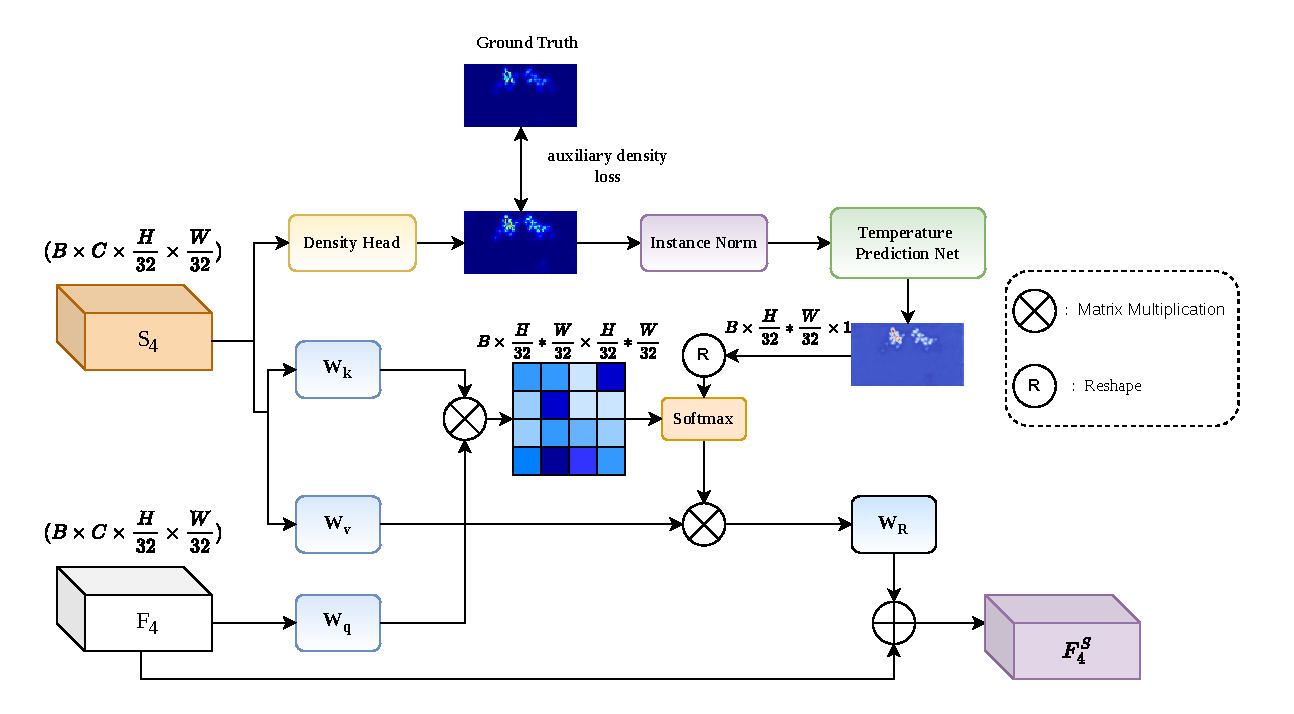
\includegraphics[width=0.48\textwidth]{dgfa.pdf}
  \caption{Density-Guided Frequency Attention (DGFA) at scale $l$. The spatial feature $\mathbf{S}_l$ predicts an auxiliary density prior, whose normalized relative density layout is transformed into a query-wise temperature map. The frequency feature $\widetilde{\mathbf{F}}_l$ provides the queries, while the keys and values are projected from $\mathbf{S}_l$. The density-conditioned temperature adaptively controls the concentration of spatial-to-frequency cross-attention, producing $\mathbf{F}_l^{S}$.}
  \label{fig:4}
  \vspace{-1em}
\end{figure}
%, applied to feature $F_{target}$ using $F_{sourse}$
\vspace{-1em}

\subsection{Density-Guided Frequency Attention}
\label{DGFA}
Although the spatial-frequency pathway preserves complementary structural and detail information, its representation may lack explicit crowd-location semantics. We therefore introduce Density-Guided Frequency Attention (DGFA), which performs spatial-to-frequency cross-attention with a density-conditioned temperature. Unlike conventional cross-attention with a globally fixed logit scale, DGFA uses the relative density layout predicted from the spatial feature to adaptively control the attention concentration at each query location.

At scale $l\in\{4,3\}$, let $\widetilde{\mathbf F}_{l},\mathbf S_{l}\in\mathbb R^{B\times C_l\times H_l\times W_l}$ denote the input frequency feature and the spatial feature, respectively, where $N_l=H_lW_l$. At the first refinement scale, $\widetilde{\mathbf F}_{4}=\mathbf F_{4}$; at the second scale, $\widetilde{\mathbf F}_{3}$ is obtained by projecting and upsampling the fused stage-4 representation.

We first estimate an auxiliary density response from the spatial feature:
\begin{equation}
\hat{\mathbf D}_{t,l}^{\mathrm{aux}}=\mathcal H_l^{\mathrm{aux}}(\mathbf S_l),
\qquad
\hat{\mathbf D}_{t,l}^{\mathrm{aux}}\in\mathbb R^{B\times1\times H_l\times W_l}.
\label{eq:aux_density}
\end{equation}
The auxiliary response is supervised by the resized ground-truth density map in Section~\ref{ls}. We then apply instance normalization to emphasize its relative spatial layout and generate the adaptive temperature map using two $1\times1$ convolutions with a GELU activation:
\begin{equation}
\boldsymbol{\tau}_l
=
\sigma\!\left(
\mathcal G_l\!\left[
\operatorname{IN}\!\left(\hat{\mathbf D}_{t,l}^{\mathrm{aux}}\right)
\right]
\right),
\label{eq:temperature}
\end{equation}
where $\sigma(\cdot)$ is the sigmoid function. After flattening the spatial dimensions, $\boldsymbol{\tau}_l\in\mathbb R^{B\times N_l\times1}$ and is broadcast along the key dimension.

The query is projected from the frequency representation, while the key and value are projected from the spatial representation:
\begin{equation}
\begin{aligned}
\mathbf Q_l &= \operatorname{Vec}\!\left(W_l^q(\widetilde{\mathbf F}_l)\right),\\
\mathbf K_l &= \operatorname{Vec}\!\left(W_l^k(\mathbf S_l)\right),\\
\mathbf V_l &= \operatorname{Vec}\!\left(W_l^v(\mathbf S_l)\right),
\end{aligned}
\label{eq:qkv_dgfa}
\end{equation}
where $\mathbf Q_l,\mathbf K_l,\mathbf V_l\in\mathbb R^{B\times N_l\times d_l}$. The density-conditioned attention is computed as
\begin{equation}
\mathbf A_l
=
\operatorname{Softmax}_{k}\!\left[
\left(s_l\mathbf Q_l\mathbf K_l^{\top}\right)
\oslash
\boldsymbol{\tau}_l
\right],
\label{eq:dgfa_attention}
\end{equation}
where $s_l$ is a learnable scale, $\oslash$ denotes broadcast division, and the Softmax is applied along the key dimension. Thus, the density-conditioned temperature controls the attention entropy separately for each frequency-domain query location.

Finally, the aggregated spatial information is projected back to the original layout and added through a residual connection:
\begin{equation}
\mathbf F_l^{S}
=
\widetilde{\mathbf F}_l
+
W_l^o\!\left[
\operatorname{Unvec}\!\left(\mathbf A_l\mathbf V_l\right)
\right].
\label{eq:dgfa_output}
\end{equation}
DGFA is applied at the two coarse feature scales, $H/32\times W/32$ and $H/16\times W/16$, to introduce density-conditioned global spatial context while limiting the quadratic cost of the attention matrix.

\begin{figure}
  \centering  
  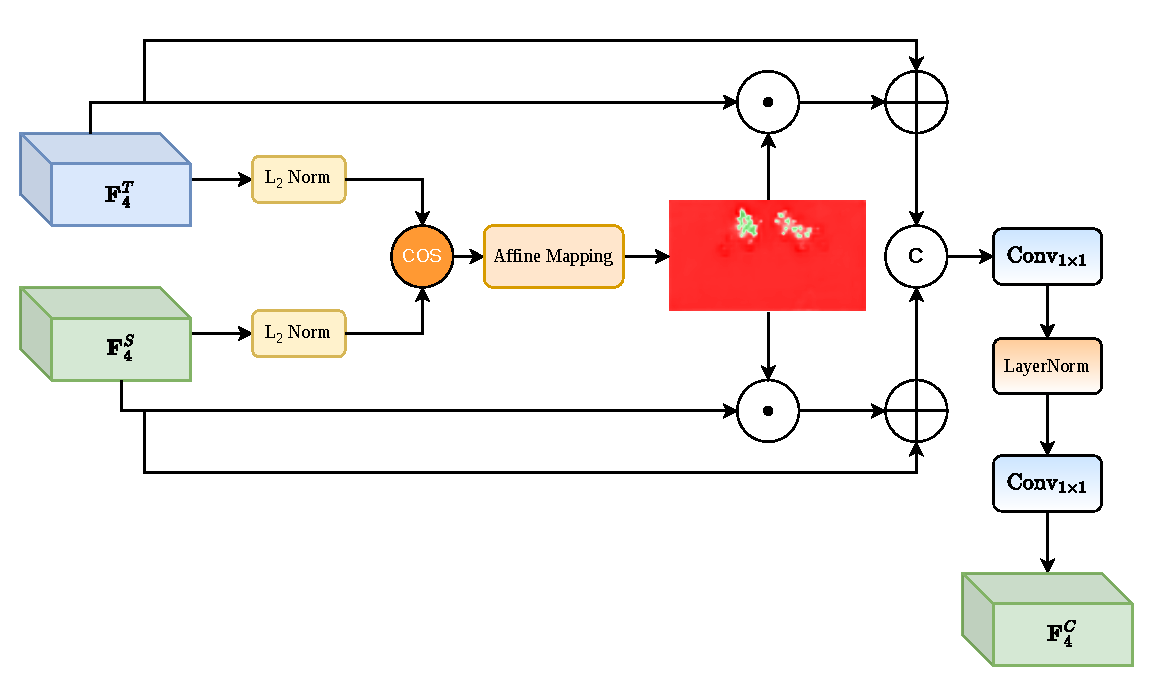
\includegraphics[width=0.48\textwidth]{DSE.pdf}
  \caption{Dual-Domain Similarity Enhancement (DSE). The temporal-frequency representation $\mathbf{F}_{l}^{T}$ and spatially guided frequency representation $\mathbf{F}_{l}^{S}$ are normalized channel-wise to compute a pixel-wise cross-branch agreement map. The mapped agreement scores assign larger residual amplification factors to locations with higher similarity, after which the enhanced features are concatenated and projected to obtain $\mathbf{F}_{l}^{C}$.}
  \label{fig:5}
  \vspace{-1em}
\end{figure}
\vspace{-1em}

%, followed by layer normalization
\subsection{Dual-Domain Similarity Enhancement}
\label{fuse}
At each refinement scale, TFRM and DGFA enhance the same frequency representation from complementary temporal and spatial perspectives, producing $\mathbf F_l^{T}$ and $\mathbf F_l^{S}$, respectively. Direct concatenation treats all responses equally and does not distinguish locations where the two pathways provide mutually supported evidence. We therefore introduce Dual-Domain Similarity Enhancement (DSE), which assigns larger residual enhancement factors to locations with stronger cross-branch agreement while preserving the complete information of both pathways.

For each spatial position $p$, the two branch features are normalized along the channel dimension, and their cosine agreement is computed as
\begin{equation}
\mathbf M_l^{\mathrm{raw}}(p)
=
\frac{
\left\langle
\mathbf F_{l,:,p}^{T},
\mathbf F_{l,:,p}^{S}
\right\rangle
}{
\left\|\mathbf F_{l,:,p}^{T}\right\|_2
\left\|\mathbf F_{l,:,p}^{S}\right\|_2
+\varepsilon
},
\qquad
\mathbf M_l^{\mathrm{raw}}(p)\in[-1,1].
\label{eq:dse_cos}
\end{equation}
A fixed affine mapping converts the agreement score to $[0,1]$:
\begin{equation}
\mathbf M_l
=
\frac{\mathbf M_l^{\mathrm{raw}}+1}{2}.
\label{eq:dse_gate}
\end{equation}
The mapped score monotonically assigns larger amplification factors to locations with higher cross-branch similarity. It is broadcast along the channel dimension and applied through residual enhancement:
\begin{equation}
\begin{aligned}
\hat{\mathbf F}_l^{T}
&=
\mathbf F_l^{T}\odot(1+\mathbf M_l),\\
\hat{\mathbf F}_l^{S}
&=
\mathbf F_l^{S}\odot(1+\mathbf M_l).
\end{aligned}
\label{eq:dse_enhance}
\end{equation}
The factor $1+\mathbf M_l$ preserves every response while assigning stronger amplification to highly agreed locations. The enhanced features are concatenated and projected to obtain the fused representation:
\begin{equation}
\mathbf F_l^{C}
=
W_l^{2}\!\left[
\operatorname{LN}\!\left(
W_l^{1}\!\left[
\operatorname{Concat}\!\left(
\hat{\mathbf F}_l^{T},
\hat{\mathbf F}_l^{S}
\right)
\right]
\right)
\right],
\label{eq:dse_fusion}
\end{equation}
where $W_l^{1}$ compresses the concatenated channels, $\operatorname{LN}(\cdot)$ denotes LayerNorm, and $W_l^{2}$ restores the output channel dimension. The stage-4 fused feature is projected and upsampled to provide top-down information for stage-3 refinement. The stage-3 output is subsequently projected and upsampled before being fed into the density regression head. In this manner, DSE reinforces reliable cross-branch agreement without discarding the complementary responses of either pathway.

\subsection{Training Objective}
\label{ls}
The proposed network is trained using a primary density regression loss, an auxiliary density-prior loss for DGFA, and a supervised density-variation loss between adjacent predictions. The complete objective is
\begin{equation}
\mathcal L
=
\mathcal L_{\mathrm{den}}
+
\lambda_a\mathcal L_{\mathrm{aux}}
+
\lambda_t\mathcal L_{\mathrm{var}},
\label{eq:total_loss}
\end{equation}
where $\lambda_a$ and $\lambda_t$ balance the two auxiliary objectives.

Given the predicted density map $\hat{\mathbf D}_t$ and ground-truth density map $\mathbf D_t$ of frame $t$, the primary regression loss is
\begin{equation}
\mathcal L_{\mathrm{den}}
=
\sum_{i=1}^{H_D}\sum_{j=1}^{W_D}
\left(
\hat{\mathbf D}_t(i,j)-\mathbf D_t(i,j)
\right)^2.
\label{eq:density_loss}
\end{equation}

DGFA predicts auxiliary density responses from the stage-4 and stage-3 spatial features. Let $\hat{\mathbf D}_{t}^{s4}$ and $\hat{\mathbf D}_{t}^{s3}$ denote these predictions. Their direct supervision is defined as
\begin{equation}
\mathcal L_{\mathrm{aux}}
=
\left\|
\hat{\mathbf D}_{t}^{s4}-\mathcal R_{s4}(\mathbf D_t)
\right\|_1
+
\left\|
\hat{\mathbf D}_{t}^{s3}-\mathcal R_{s3}(\mathbf D_t)
\right\|_1,
\label{eq:aux_loss}
\end{equation}
where $\mathcal R_{s4}(\cdot)$ and $\mathcal R_{s3}(\cdot)$ resize the ground-truth density map to the corresponding feature resolutions. This auxiliary supervision encourages the spatial pathway to provide informative crowd-distribution priors for density-conditioned attention.

To regularize the evolution of adjacent predictions without forcing them to be identical, we match the predicted density variation with the corresponding ground-truth variation:
\begin{equation}
\Delta\hat{\mathbf D}_t
=
\hat{\mathbf D}_t-\hat{\mathbf D}_{t-1},
\qquad
\Delta\mathbf D_t
=
\mathbf D_t-\mathbf D_{t-1}.
\end{equation}
The supervised density-variation loss is
\begin{equation}
\mathcal L_{\mathrm{var}}
=
\frac{1}{H_DW_D}
\sum_{i=1}^{H_D}\sum_{j=1}^{W_D}
\left|
\Delta\hat{\mathbf D}_t(i,j)-\Delta\mathbf D_t(i,j)
\right|.
\label{eq:variation_loss}
\end{equation}
Unlike a direct smoothness constraint, this objective preserves legitimate temporal changes by requiring the predicted variation to follow the annotated density evolution. The same network parameters are used to generate the adjacent predictions; the previous prediction is used by the loss rather than propagated as an input to the current estimation.

\section{Experiments}
\subsection{Experimental Setup}
\label{ID}
\textbf{Datasets.}
We evaluate WaveLoop on five public video crowd counting benchmarks: Bus~\cite{ling2023motional}, Classroom~\cite{ling2023motional}, Mall~\cite{chen2012feature}, Venice~\cite{liu2019context}, and FDST~\cite{fang2019locality}. These datasets cover indoor and outdoor surveillance scenes with different crowd-density ranges, occlusion patterns, viewpoints, and temporal dynamics. We follow the official training and test protocols of each dataset. For model selection, the last 10\% of the training sequences are reserved for validation.

\textbf{Implementation details.}
Following MFA~\cite{ling2023motional} and DACM~\cite{ling2025dual}, we apply random cropping and horizontal flipping with a probability of $0.5$. ConvNeXt-T~\cite{liu2022convnet} and the lightweight ConvNeXt-Atto encoders~\cite{woo2023convnext} are initialized with ImageNet-22K and ImageNet-1K pre-trained weights, respectively. The network is optimized using AdamW with a weight decay of $1\times10^{-4}$. The initial learning rate is $5\times10^{-6}$ on Bus, Classroom, Mall, and FDST, and $1\times10^{-4}$ on Venice. The loss weights $\lambda_a$ and $\lambda_t$ are both set to $1$. All experiments are implemented in PyTorch and conducted on a single NVIDIA GeForce RTX 5090 GPU.

\subsection{Evaluation Metrics}
Following previous video crowd counting studies~\cite{wu2022spatial,dong2022clrnet,hou2023frame}, we use Mean Absolute Error (MAE) and Root Mean Squared Error (RMSE) to evaluate frame-level counting accuracy. For the $z$-th test frame, the estimated count is obtained by summing the predicted density map:
\begin{equation}
N_z=\sum_{i=1}^{H_z}\sum_{j=1}^{W_z}\hat{\mathbf D}_z(i,j).
\end{equation}
MAE and RMSE are defined as
\begin{equation}
\begin{aligned}
\mathrm{MAE}
&=
\frac{1}{Z}\sum_{z=1}^{Z}\left|N_z-N_z^{\mathrm{gt}}\right|,\\
\mathrm{RMSE}
&=
\sqrt{\frac{1}{Z}\sum_{z=1}^{Z}\left(N_z-N_z^{\mathrm{gt}}\right)^2},
\end{aligned}
\label{eq:count_metrics}
\end{equation}
where $Z$ is the number of test frames, and $N_z^{\mathrm{gt}}$ and $N_z$ are the ground-truth and estimated counts, respectively. MAE measures the average counting deviation, whereas RMSE assigns larger penalties to frames with large errors.

\subsection{Comparison with the State-of-the-Art Methods}
We compare WaveLoop with representative image-based and video-based crowd counting methods on the five benchmarks. Image-based methods estimate each frame independently, whereas video-based methods exploit temporal information through recurrent modeling, multi-frame aggregation, explicit motion cues, or spatiotemporal interaction. Overall, WaveLoop achieves the lowest MAE on all five datasets and the lowest or second-lowest RMSE across the benchmarks. These results support the effectiveness of jointly modeling current-frame spatial-frequency representations, temporally shared context, rapid inter-frame variations, and density-guided spatial semantics. The contribution of each component is examined separately in Section~\ref{sec:ablation}; the following comparisons therefore focus on the complete framework rather than attributing a dataset-specific improvement to one module.

\begin{table}[h]
\caption{Quantitative comparisons on the Bus and Classroom datasets. The best and second-best results are highlighted in \textbf{bold} and \underline{underline}, respectively. Tied best results are all highlighted in bold.}
\centering
\scriptsize
\begin{tabular}{cccccc}
    \toprule
    \multirow{2}{*}{Category}&Dataset&\multicolumn{2}{c}{Bus}&\multicolumn{2}{c}{Classroom}\\
    &Method &MAE & RMSE&MAE & RMSE\\
    \midrule
     %& CSRNet \cite{li2018csrnet} & 1.99 & 2.40 & 3.42 & 3.86 \\
   Image & CAN \cite{liu2019context} & 2.25 & 2.69 & 1.72 & 2.09 \\
   & Bayesian \cite{ma2019bayesian} &3.03 & 3.70 & 2.86 & 3.14 \\
   & RR \cite{wan2019residual} &  1.67 & 2.03 & 4.07 & 4.38 \\
   & KDMG \cite{wan2020kernel} &  2.43 & 2.92 & 4.17 & 4.48 \\
   & DMCount \cite{wang2020distribution} & 2.37 & 2.95 & 2.86 & 3.49 \\
   & TopoCount \cite{abousamra2021localization}  & 2.69 & 3.44 & 2.75 & 3.34 \\
   & P2PNet \cite{song2021rethinking}  & 4.28 & 5.26 & 1.63 & 2.08 \\ 
   & MAN \cite{lin2022boosting} & 2.75 & 3.28 & 2.35 & 2.72 \\ 
   & ConvNeXt \cite{liu2022convnet}  & 1.65 & 2.01 & 3.17 & 3.93 \\
   & CHS-Net \cite{dai2023cross} & 1.81 & 2.19 & 1.46 & 1.80 \\
   & HMoDE \cite{du2023redesigning} & 1.77 & 2.13 & 1.49 & 1.95 \\  
   & Gramformer \cite{lin2024gramformer}  & 2.25 & 2.62 & 1.65 & 2.07 \\  
   \midrule
   Video & LSTN \cite{fang2019locality} &  2.47 & 3.13 & 3.02 & 3.90 \\
   & EPF \cite{liu2020estimating} & 1.69 & 2.08 & 2.16 & 2.48 \\
   & STGN \cite{wu2022spatial} & 1.58 & 1.92 & 1.54 & 1.83 \\
   & MFA \cite{ling2023motional} & 1.42 & 1.80 & 1.64 & 2.00 \\ 
   & DACM \cite{ling2025dual} & \underline{1.32} & \textbf{1.66} & 1.70 & 2.03 \\ 
   & DSTI \cite{ling2026dual} & \underline{1.32} & \underline{1.68} & \underline{1.42} & \underline{1.71}  \\
   & WaveLoop  & \textbf{1.30} & \textbf{1.66} & \textbf{1.30} & \textbf{1.54} \\
    \bottomrule
\end{tabular}
\label{tab:1}
 \vspace{-1em}
\end{table}

\textit{1) Bus and Classroom.}
Table~\ref{tab:1} reports the results on the two indoor benchmarks. On Bus, WaveLoop achieves an MAE/RMSE of 1.30/1.66. Compared with ConvNeXt~\cite{liu2022convnet}, the strongest image-based baseline on this dataset, WaveLoop reduces MAE and RMSE by 21.2\% and 17.4\%, respectively. Among video-based competitors, WaveLoop improves the best competing MAE from 1.32 to 1.30 and ties DACM~\cite{ling2025dual} for the lowest RMSE of 1.66. Although the MAE improvement is modest, the result shows that the complete framework remains competitive on Bus without sacrificing the sensitivity to difficult frames measured by RMSE.

On Classroom, WaveLoop obtains an MAE of 1.30 and an RMSE of 1.54, outperforming all compared image- and video-based methods. Relative to CHS-Net~\cite{dai2023cross}, the strongest image-based method, the proposed method reduces MAE and RMSE by 11.0\% and 14.4\%, respectively. Compared with DSTI~\cite{ling2026dual}, the strongest video-based competitor on both metrics, WaveLoop yields relative reductions of 8.5\% in MAE and 9.9\% in RMSE. The simultaneous improvement in both metrics indicates that WaveLoop reduces the average frame-level error while also suppressing large errors in challenging classroom frames. This performance is consistent with the design objective of combining stable temporal context, motion-sensitive variations, and density-guided spatial-frequency interaction; the respective effects of TFRM, DGFA, and DSE are verified in the ablation study rather than inferred solely from this comparison.

\begin{table}[h]
\caption{Quantitative comparisons on the FDST dataset. The best and second-best results are highlighted in \textbf{bold} and \underline{underline}, respectively. MFA$^{*}$ denotes the result reproduced using the official implementation at an input resolution of $640\times360$.}
\centering
\scriptsize
\begin{tabular}{@{}cccc@{}}
\toprule
Category & Method & MAE & RMSE  \\ 
\midrule
 %& CSRNet \cite{li2018csrnet} & 2.56 & 3.12 \\
Image & Bayesian \cite{ma2019bayesian} & 2.85 & 3.74 \\
& CAN \cite{liu2019context} & 2.44 & 2.96 \\
& ADCrowdNet \cite{liu2019adcrowdnet} & 2.18 & 2.84 \\
& RPNet \cite{yang2020reverse} & 2.38 & 3.03 \\
& Gramformer \cite{lin2024gramformer} & 5.15 & 6.32 \\
\midrule
 %& Bi-ConvLSTM \cite{xiong2017spatiotemporal}  & 4.48 & 5.82 \\
Video & LSTN \cite{fang2019locality} & 3.35 & 4.45 \\
& EPF \cite{liu2020estimating} & 2.10 & 2.46 \\
& MOPN \cite{hossain2020video}  & 1.76 & 2.25 \\
& PHNet \cite{meng2021phnet} & 1.65 & 2.16 \\
& GNANet \cite{li2022video} & 2.10 & 2.90 \\
& GRGAF-ST \cite{cai2022global} & 1.91 & 2.45 \\
& CLRNet \cite{dong2022clrnet} & 1.45 & 1.97 \\
& MFA* \cite{ling2023motional} & 1.90 & 2.60 \\
& FRVCC \cite{hou2023frame} & 1.62 & 2.36 \\
& STGN \cite{wu2022spatial} & {1.38} & {1.82} \\
& SSCR \cite{yong2025lightweight} & 2.06 & 2.53 \\
& DACM \cite{ling2025dual} & 1.31 & 1.75 \\
& E-MAC \cite{cao2024efficient} & 1.29 & 1.69 \\
& DSTI \cite{ling2026dual} & 1.33 & 1.71 \\
& CCINet \cite{ling2026cascaded} & \underline{1.25} & \textbf{1.62} \\
& WaveLoop  & \textbf{1.16} & \underline{1.64} \\
\bottomrule
\end{tabular}
\label{tab:2}
 \vspace{-1em}
\end{table}

\textit{2) FDST.}
FDST contains diverse indoor and outdoor scenes and therefore provides a comprehensive evaluation of scene adaptability. As shown in Table~\ref{tab:2}, WaveLoop is compared with five image-based methods and fifteen existing video-based methods. The reproduced MFA result, denoted by MFA$^{*}$, is obtained using its official implementation with an input resolution of $640\times360$.

WaveLoop achieves the lowest MAE of 1.16 and the second-lowest RMSE of 1.64. Compared with ADCrowdNet~\cite{liu2019adcrowdnet}, the strongest image-based method in the table, WaveLoop reduces MAE and RMSE by 46.8\% and 42.3\%, respectively. Compared with CCINet~\cite{ling2026cascaded}, WaveLoop further reduces MAE from 1.25 to 1.16, corresponding to a relative improvement of 7.2\%. Its RMSE is 1.64, which is slightly higher than the 1.62 obtained by CCINet. This result indicates that WaveLoop improves the average counting accuracy across diverse scenes, while a small number of difficult frames still produce relatively large errors. Reporting per-scene results or error-distribution plots would further clarify where these large errors occur.

Figure~\ref{fig:6} presents qualitative predictions on representative indoor and outdoor FDST scenes. The predicted density maps preserve the main crowd regions and remain spatially aligned with the ground-truth distributions under different scene layouts. In the outdoor examples, the model responds to pedestrians distributed over a broad area, whereas in the indoor examples it maintains concentrated responses in heavily occluded regions while suppressing most background areas. These visualizations support the quantitative results by showing that the complete model can produce localized density responses across diverse scenes. Since Fig.~\ref{fig:6} does not include competing methods, it should be interpreted as a qualitative inspection of WaveLoop rather than a cross-method visual comparison.

\begin{figure*}[t]
\centering

\subfloat[]{
    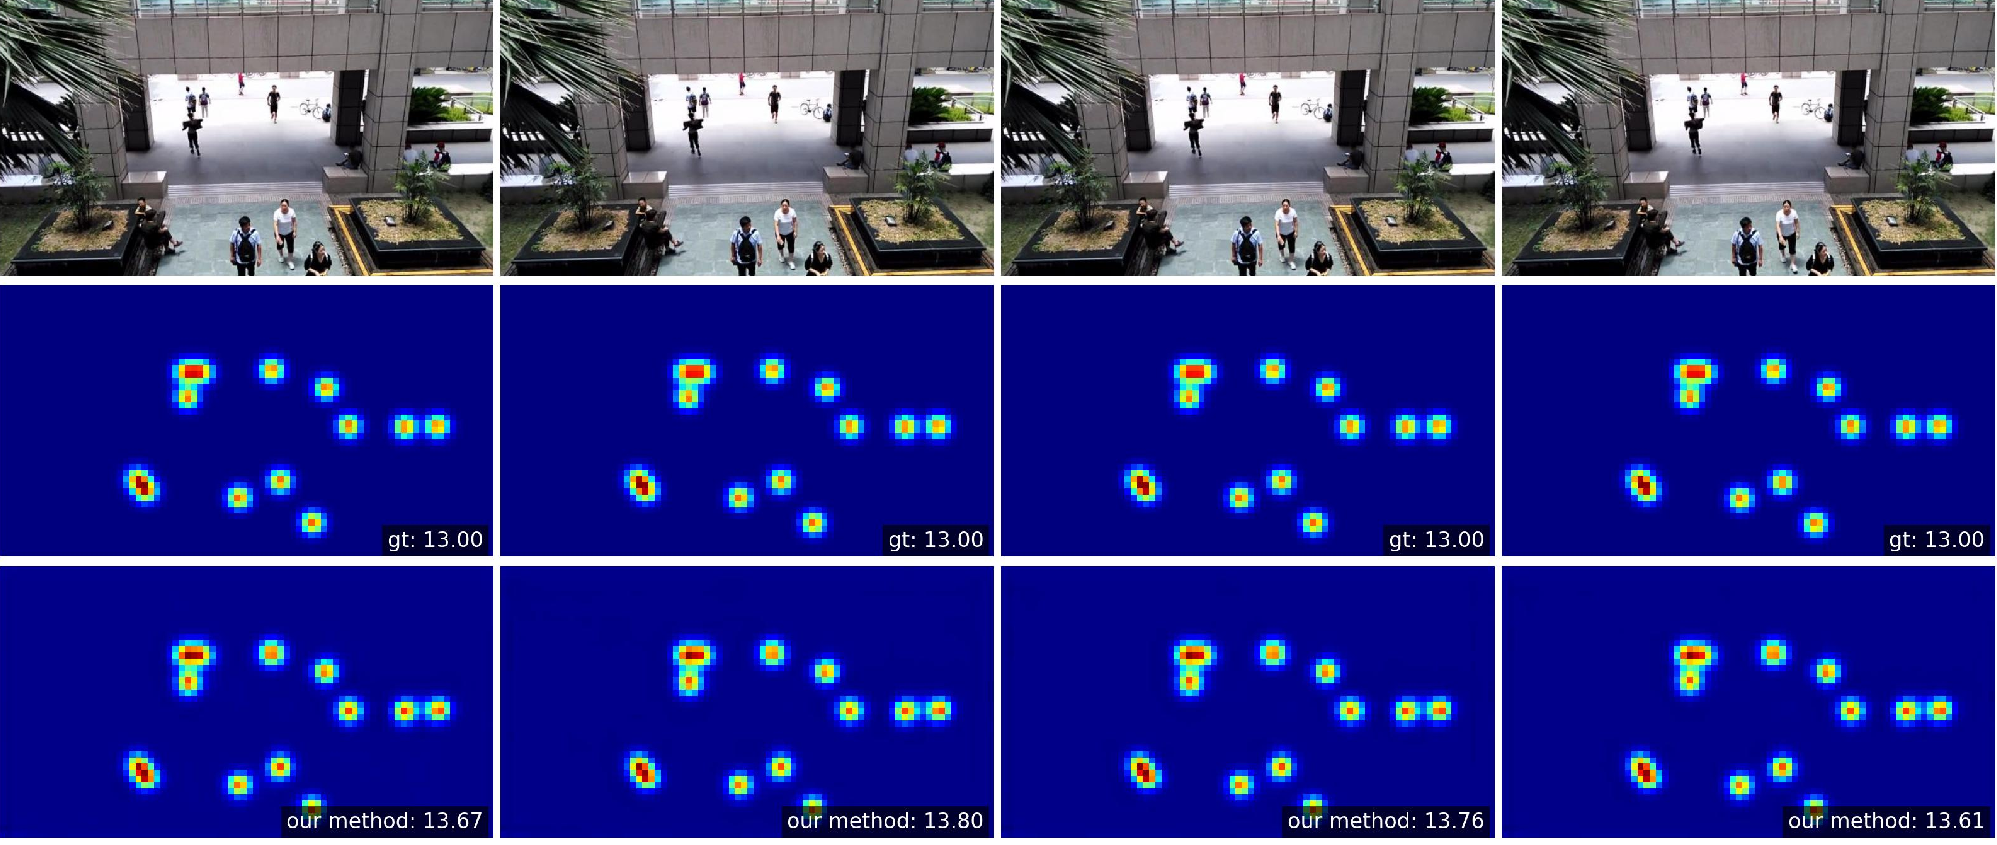
\includegraphics[width=0.47\textwidth]{outdoor1.pdf}}
\hfill
\subfloat[]{
    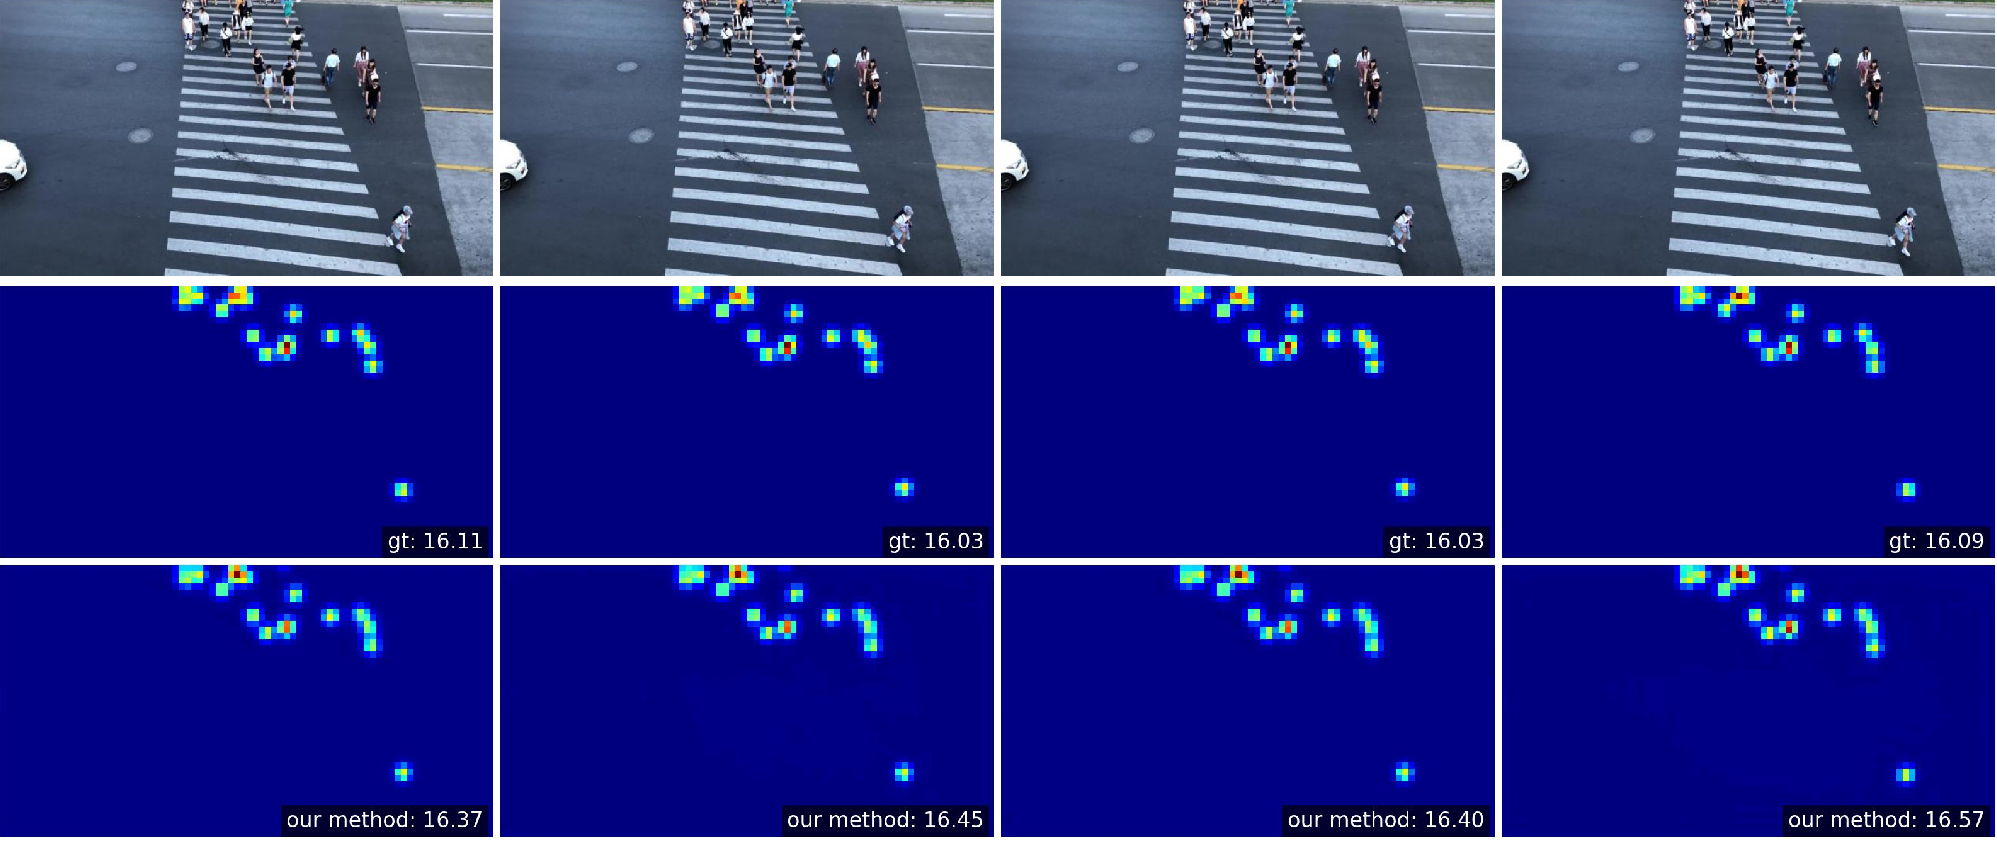
\includegraphics[width=0.47\textwidth]{outdoor2.pdf}}
\\[0.2em]

\subfloat[]{
    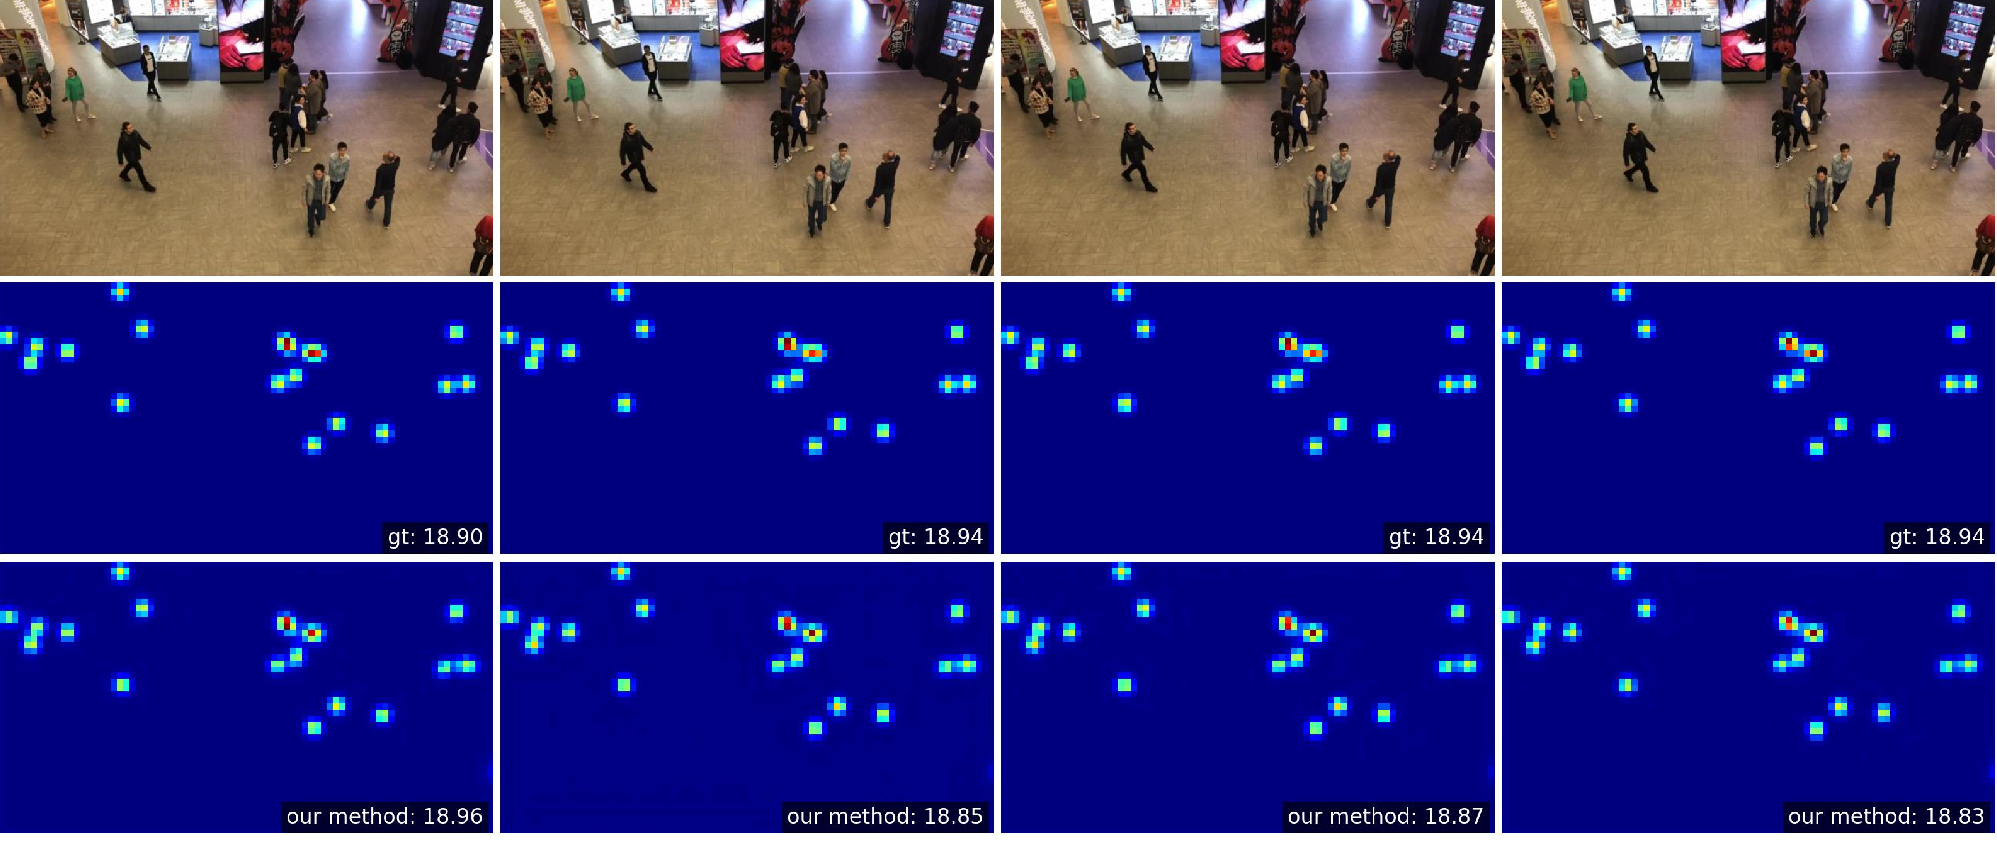
\includegraphics[width=0.47\textwidth]{indoor1.pdf}}
\hfill
\subfloat[]{
    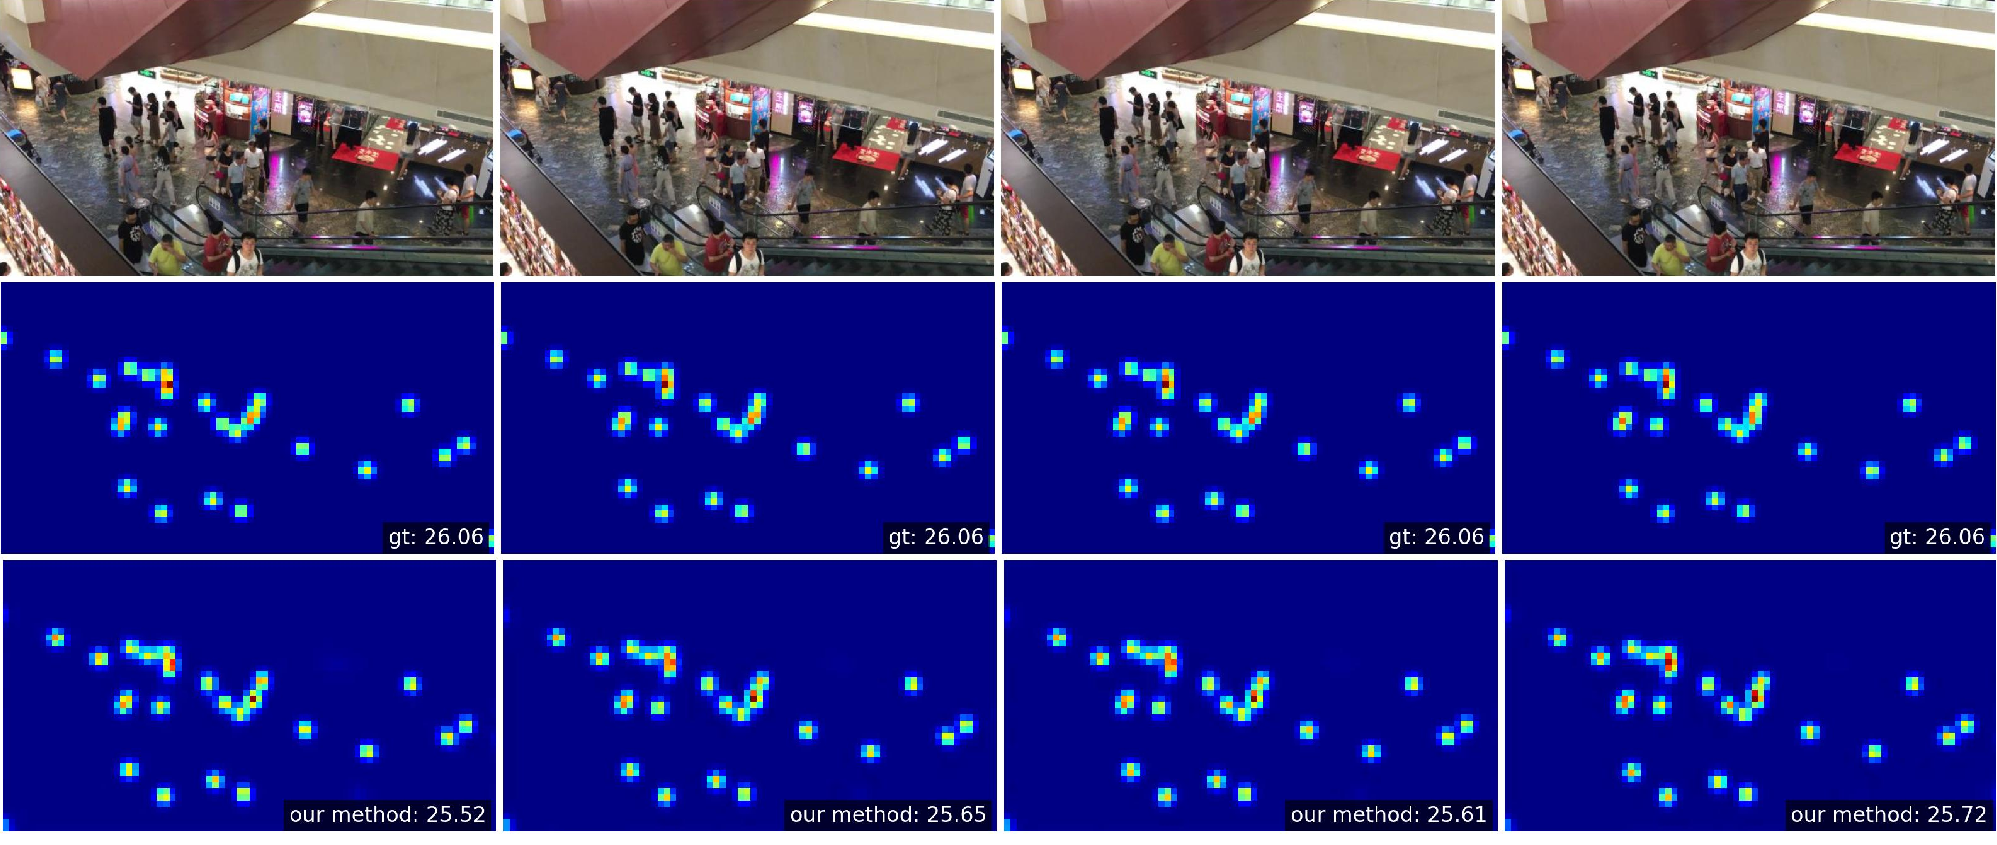
\includegraphics[width=0.47\textwidth]{indoor2.pdf}}

\caption{Qualitative results of WaveLoop on representative FDST scenes. The first row shows the input frames, the second row presents the ground-truth density maps, and the third row shows the corresponding predictions. Panels (a)--(b) are outdoor scenes, while panels (c)--(d) are indoor scenes.}
\label{fig:6}
\vspace{-1em}
\end{figure*}

\begin{table}[h]
\caption{Quantitative comparisons on the Mall dataset. The best and second-best results are highlighted in \textbf{bold} and \underline{underline}, respectively.}
\centering
\scriptsize
\begin{tabular}{@{}cccc@{}}
\toprule
Category & Method & MAE & RMSE  \\ 
\midrule
Image & RR \cite{wan2019residual}  & 2.52 & 3.09 \\
& Bayesian \cite{ma2019bayesian}  & 1.96 & 2.49 \\ 
& ADCrowdNet \cite{liu2019adcrowdnet}  & 1.92 & 2.45 \\
& KDMG \cite{wan2020kernel}  & 2.35 & 2.92 \\
& RPNet \cite{yang2020reverse}  & 2.20 & 3.60 \\
& DMCount \cite{wang2020distribution}  & 2.02 & 2.52 \\
& MAN \cite{lin2022boosting}  & 2.14 & 2.71 \\
& ConvNeXt \cite{liu2022convnet}  & 1.62 & 2.02 \\
& CHS-Net \cite{dai2023cross}  & 1.71 & 2.18 \\
& HMoDE \cite{du2023redesigning}  & 1.70 & 2.14 \\
& Gramformer \cite{lin2024gramformer}  & 1.69 & 2.14 \\
\midrule
Video & LSTN \cite{fang2019locality}  &2.00 & 2.50 \\
& E3D \cite{zou2019enhanced}  & 1.64 & 2.13 \\
& MOPN \cite{hossain2020video}  & 1.78 & 2.25 \\
& GRGAF-ST \cite{cai2022global}  &1.61 & 2.07 \\
& STGN \cite{wu2022spatial}  & 1.53 & 1.97 \\
& MFA \cite{ling2023motional}  & 1.51 & 1.93 \\
& DACM \cite{ling2025dual}  & \underline{1.44} & \underline{1.85} \\
& DSTI \cite{ling2026dual}  & 1.51 & 1.92 \\
& WaveLoop & \textbf{1.36}& \textbf{1.71}\\
\bottomrule
\end{tabular}
\label{tab:3}
\vspace{-1em}
\end{table}

\textit{3) Mall.}
Mall contains continuous pedestrian flows, frequent occlusions, and substantial perspective variation under a fixed surveillance camera. As reported in Table~\ref{tab:3}, WaveLoop achieves the best MAE and RMSE, with values of 1.36 and 1.71, respectively. Compared with ConvNeXt~\cite{liu2022convnet}, the strongest image-based baseline, WaveLoop reduces MAE by 16.0\% and RMSE by 15.3\%. This gap confirms that exploiting adjacent-frame information provides additional cues beyond single-frame appearance.

Compared with DACM~\cite{ling2025dual}, the strongest video-based competitor, WaveLoop further reduces MAE and RMSE by 5.6\% and 7.6\%, respectively. The gains on both metrics are consistent with the overall design of WaveLoop, which separates temporally shared information from rapid inter-frame variations and then coordinates these temporal-frequency cues with the current-frame spatial representation. Nevertheless, the causal contribution of each operation is established by the controlled component analysis rather than by the state-of-the-art comparison alone.

\begin{table}[h]
\caption{Quantitative comparisons on the Venice dataset. The best and second-best results are highlighted in \textbf{bold} and \underline{underline}, respectively.}
\centering
\scriptsize
\begin{tabular}{@{}cccc@{}}
\toprule
Category & Method & MAE & RMSE  \\ 
\midrule
 %& CSRNet \cite{li2018csrnet} & 35.8 & 50.0 \\
Image & ADCrowdNet \cite{liu2019adcrowdnet} & 24.2 & 40.1 \\
& CAN \cite{liu2019context} & 23.5 & 38.9 \\
& ECAN \cite{liu2019context} & 20.5 & 29.9 \\
& RPNet \cite{yang2020reverse} & 26.3 & 43.3 \\
& Gramformer \cite{lin2024gramformer} & 21.3 & 28.6 \\
%& EHNET \cite{yan2025ehnet} & 22.4 & 32.2 \\
\midrule
Video & EPF \cite{liu2020estimating} & 15.0 & 19.6 \\
& PHNet \cite{meng2021phnet} & 18.1 & 25.1 \\
& STGN \cite{wu2022spatial} & 14.1 & 20.1 \\
& FRVCC \cite{hou2023frame}  & {13.2} & {16.5} \\
& DACM \cite{ling2025dual} & \underline{11.1} & \underline{14.3} \\
& DSTI \cite{ling2026dual} & 11.6 & 14.8 \\
& WaveLoop  & \textbf{10.4} & \textbf{14.2} \\
\bottomrule
\end{tabular}
\label{tab:4}
\vspace{-1em}
\end{table}

\textit{4) Venice.}
Venice is particularly challenging because of its limited training data and the substantial viewpoint discrepancy between the training and test sequences. As shown in Table~\ref{tab:4}, WaveLoop obtains the best MAE/RMSE of 10.4/14.2 among all compared methods. Relative to Gramformer~\cite{lin2024gramformer}, the strongest image-based method in the table, WaveLoop reduces MAE and RMSE by 51.2\% and 50.3\%, respectively, demonstrating the clear advantage of exploiting video information in this setting.

Compared with DACM~\cite{ling2025dual}, WaveLoop reduces MAE from 11.1 to 10.4, corresponding to a relative improvement of 6.3\%, while RMSE decreases slightly from 14.3 to 14.2. The larger improvement in MAE than in RMSE suggests that WaveLoop improves the typical frame-level prediction but provides only a limited reduction in the largest errors. The overall result is consistent with the intended role of the wavelet-based representation in retaining complementary structural and detail cues under limited training data. However, SAFF should not be identified as the sole cause of this improvement unless a Venice-specific module ablation is additionally provided.

\subsection{Ablation and Diagnostic Studies}
\label{sec:ablation}

\subsubsection{Cumulative Component Analysis}
We first evaluate the cumulative contribution of the proposed components on the Classroom dataset. As reported in Table~\ref{tab:component_ablation}, the ConvNeXt-T baseline obtains an MAE of 1.93 and an RMSE of 2.32. Introducing SAFF reduces MAE and RMSE to 1.60 and 1.87, respectively, while adding only 0.6M parameters. This result supports the motivation of calibrating the magnitude discrepancy among spatial wavelet bands before frequency aggregation.

On top of SAFF, TFRM further reduces MAE/RMSE from 1.60/1.87 to 1.56/1.79. The improvement is consistent with the intended role of TFRM in adapting current-frame frequency features using temporally shared content and rapid inter-frame variations. Incorporating DGFA yields an additional improvement to 1.51/1.73, indicating that density-conditioned spatial guidance facilitates the coordination of spatial and frequency-domain representations. Finally, DSE reduces MAE/RMSE to 1.30/1.54 by assigning stronger enhancement to highly agreed responses from the temporal-frequency and spatial-frequency pathways before fusion.

Overall, the complete model improves MAE and RMSE by 32.6\% and 33.6\%, respectively, over the baseline. Because the modules are introduced cumulatively, the results demonstrate their incremental effectiveness under the complete design path rather than fully isolated contributions. Additional mechanism-specific comparisons are therefore provided in the following diagnostic studies.

\begin{table}[t]
\caption{Cumulative component analysis on the Classroom dataset. ``P'' denotes the number of parameters.}
\centering
\scriptsize
\setlength{\tabcolsep}{3pt}
\begin{tabular}{cccccccc}
\toprule
Baseline & SAFF & TFRM & DGFA & DSE & MAE & RMSE & P (M) \\
\midrule
\checkmark &  &  &  &  & 1.93 & 2.32 & 28.0 \\
\checkmark & \checkmark &  &  &  & 1.60 & 1.87 & 28.6 \\
\checkmark & \checkmark & \checkmark &  &  & 1.56 & 1.79 & 39.3 \\
\checkmark & \checkmark & \checkmark & \checkmark &  & 1.51 & 1.73 & 41.7 \\
\checkmark & \checkmark & \checkmark & \checkmark & \checkmark & \textbf{1.30} & \textbf{1.54} & 41.9 \\
\bottomrule
\end{tabular}
\label{tab:component_ablation}
\end{table}

\subsubsection{Effect of Loss Weights}
We analyze the weights of the supervised density-variation loss, $\lambda_t$, and the auxiliary density-prior loss, $\lambda_a$, on Classroom. When varying one weight, the other is fixed to 1.0, and all remaining training settings are kept unchanged. Each weight is selected from $\{0,0.5,1.0,1.5,2.0\}$, where a value of zero removes the corresponding auxiliary objective.

As shown in Table~\ref{tab:loss_weights}, $\lambda_t=1.0$ achieves the lowest MAE/RMSE among the tested candidates. Removing density-variation supervision increases MAE/RMSE from 1.30/1.54 to 1.58/1.79, showing that variation-level supervision provides information complementary to frame-wise density regression. Assigning an excessively large weight also degrades counting accuracy, because the auxiliary temporal objective may dominate the primary density estimation task.

The auxiliary density-prior loss exhibits a similar trend. Setting $\lambda_a=0$ increases MAE/RMSE to 1.54/1.75, whereas $\lambda_a=1.0$ gives the best result in the evaluated range. We therefore use $\lambda_t=\lambda_a=1.0$ in all experiments. These results establish the selected empirical balance among the three objectives; they should not be interpreted as evidence of optimization stability unless repeated-run statistics are additionally reported.

\begin{table}[t]
\centering
\caption{Effect of the density-variation and auxiliary density-prior loss weights on Classroom. When one weight is varied, the other is fixed to 1.0.}
\scriptsize
\begin{tabular}{cccccc}
\toprule
Weight & 0 & 0.5 & 1.0 & 1.5 & 2.0 \\
\midrule
$\lambda_t$ (MAE)  & 1.58 & 1.52 & \textbf{1.30} & 1.37 & 1.62 \\
$\lambda_t$ (RMSE) & 1.79 & 1.83 & \textbf{1.54} & 1.63 & 1.94 \\
\midrule
$\lambda_a$ (MAE)  & 1.54 & 1.59 & \textbf{1.30} & 1.62 & 1.74 \\
$\lambda_a$ (RMSE) & 1.75 & 1.99 & \textbf{1.54} & 1.91 & 1.94 \\
\bottomrule
\end{tabular}
\label{tab:loss_weights}
\end{table}

\subsubsection{Transfer Learning}
We further evaluate the transferability of WaveLoop across datasets with different scene layouts, crowd-density ranges, and frame rates. Following previous studies~\cite{xiong2017spatiotemporal,ling2023motional,ling2025dual}, we consider UCSD-to-Mall and Mall-to-UCSD adaptation. The model is first trained on all labeled frames of the source domain. It is then fine-tuned using 50 labeled target-domain frames with a learning rate of $1\times10^{-6}$, following MFA~\cite{ling2023motional}. The target-domain samples are used only for fine-tuning, and no target test frames are used during model optimization.

Table~\ref{tab:cross_dataset} compares WaveLoop with four conventional transfer/counting approaches, two image-based networks, and four video-based methods. For UCSD-to-Mall, WaveLoop obtains the second-lowest MAE of 2.44, which is 0.08 higher than MOPN~\cite{hossain2020video}. For Mall-to-UCSD, WaveLoop achieves the best MAE of 1.53, improving over MOPN by 1.3\%. The results indicate that the representations learned by WaveLoop transfer effectively across datasets after limited target-domain fine-tuning, demonstrating favorable cross-dataset transferability under the adopted transfer-learning protocol.

\begin{table}[t]
\caption{Transfer-learning results between UCSD and Mall. Each model is first trained on the source dataset and then fine-tuned using 50 labeled frames from the target dataset. The best and second-best results are shown in bold and underlined, respectively.}
\centering
\scriptsize
\begin{tabular}{ccc}
\toprule
Method & UCSD $\rightarrow$ Mall & Mall $\rightarrow$ UCSD \\
 & MAE & MAE \\
\midrule
LGP~\cite{yu2005learning} & 4.36 & 3.32 \\
FA~\cite{change2013semi} & 7.47 & 4.44 \\
GPA~\cite{liu2015bayesian} & 4.18 & 2.79 \\
GPTL~\cite{liu2015bayesian} & 3.55 & 2.91 \\
MCNN~\cite{zhang2016single} & 24.25 & 11.26 \\
Bi-ConvLSTM~\cite{xiong2017spatiotemporal} & 2.63 & 1.82 \\
CSRNet~\cite{li2018csrnet} & 14.01 & 13.96 \\
MOPN~\cite{hossain2020video} & \textbf{2.36} & \underline{1.55} \\
DACM~\cite{ling2025dual} & 2.49 & 1.78 \\
CCINet~\cite{ling2026cascaded} & 2.45 & 1.65 \\
\midrule
WaveLoop & \underline{2.44} & \textbf{1.53} \\
\bottomrule
\end{tabular}
\label{tab:cross_dataset}
\end{table}

\subsubsection{Computational Complexity}
Table~\ref{tab:complexity} compares the parameter count, computational cost, inference time, and counting accuracy of WaveLoop with representative image- and video-based methods. The GFLOPs are measured using a two-frame input pair at a spatial resolution of $384\times384$. The reported inference time is the total wall-clock time for 100 inputs at $1024\times1024$ on an NVIDIA RTX 4090 GPU. Because GFLOPs and latency are evaluated at different input resolutions, they should be interpreted as separate complexity indicators rather than directly corresponding measurements.

Compared with MFA~\cite{ling2023motional}, WaveLoop reduces the number of parameters from 58.63M to 41.94M, corresponding to a 28.5\% reduction, while improving MAE/RMSE from 1.42/1.80 to 1.30/1.66 on Bus. WaveLoop requires 64.99 GFLOPs, 18.1\% more than MFA, and its measured inference time is also higher. The additional computation mainly arises from the separate encoding of current-frame spatial-frequency features and adjacent-frame temporal-frequency components, together with density-guided interaction at two feature scales. Thus, WaveLoop favors counting accuracy and parameter efficiency at the cost of moderate additional computation and latency. Developing a lighter temporal-frequency encoder and more efficient cross-domain interaction remains an important direction.

\begin{table}[t]
\caption{Complexity and accuracy comparison on Bus. P denotes parameters in millions, and IT denotes the total inference time in seconds for 100 inputs under the protocol described in the text.}
\centering
\scriptsize
\begin{tabular}{llccccc}
\toprule
Category & Method & P & GFLOPs & IT & MAE & RMSE \\
\midrule
Image & Bayesian~\cite{ma2019bayesian} & \textbf{21.50} & 60.73 & 6.19 & 3.03 & 3.70 \\
Image & MAN~\cite{lin2022boosting} & 30.96 & 59.54 & 6.92 & 2.75 & 3.28 \\
\midrule
Video & MFA~\cite{ling2023motional} & 58.63 & \textbf{55.01} & \textbf{5.23} & 1.42 & 1.80 \\
Video & WaveLoop & 41.94 & 64.99 & 7.09 & \textbf{1.30} & \textbf{1.66} \\
\bottomrule
\end{tabular}
\label{tab:complexity}
\end{table}

\subsubsection{Effect of the TFRM Kernel Size}
We investigate the spatial kernel size used to predict the offsets and modulation masks in TFRM. As shown in Table~\ref{tab:kernel_size}, a $3\times3$ kernel achieves the best MAE/RMSE of 1.30/1.54. Replacing it with a $1\times1$ kernel increases MAE and RMSE by 11.5\% and 11.0\%, respectively, indicating that neighboring frequency responses provide useful context for temporal reconfiguration. Increasing the kernel to $5\times5$ or $7\times7$ also degrades performance. A larger receptive field may incorporate less relevant responses and makes the offset prediction more difficult to optimize, while introducing additional computation. We therefore adopt a $3\times3$ kernel as the default setting.

\begin{table}[t]
\caption{Effect of the TFRM kernel size on Classroom.}
\centering
\scriptsize
\begin{tabular}{ccc}
\toprule
Kernel size & MAE & RMSE \\
\midrule
$1\times1$ & 1.45 & 1.71 \\
$3\times3$ & \textbf{1.30} & \textbf{1.54} \\
$5\times5$ & 1.33 & 1.59 \\
$7\times7$ & 1.39 & 1.65 \\
\bottomrule
\end{tabular}
\label{tab:kernel_size}
\end{table}

\subsubsection{Hyperparameter Sensitivity}
We additionally examine the learning rate and weight decay on Classroom by varying one hyperparameter at a time while keeping all other settings fixed. As shown in Fig.~\ref{fig:hyperparameters}, the lowest MAE and RMSE are obtained with a learning rate of $5\times10^{-6}$ and a weight decay of $1\times10^{-4}$. Both smaller and larger values lead to inferior results within the tested ranges. These values are therefore used as the default optimization settings.

\begin{figure}[t]
\centering
\subfloat[]{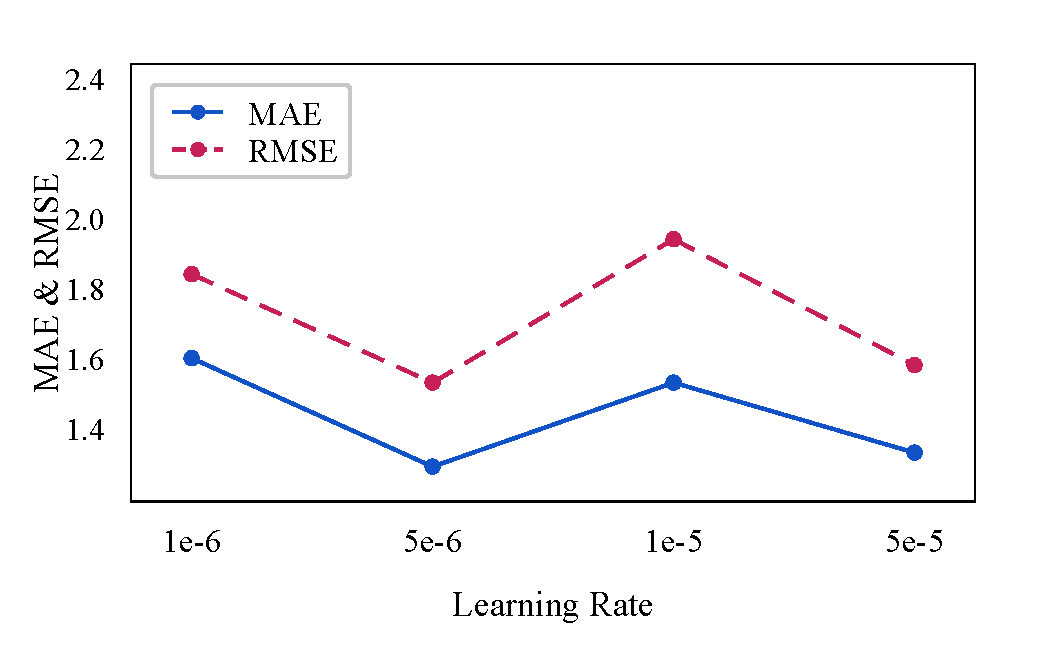
\includegraphics[height=0.31\linewidth]{lr.pdf}}
\hfill
\subfloat[]{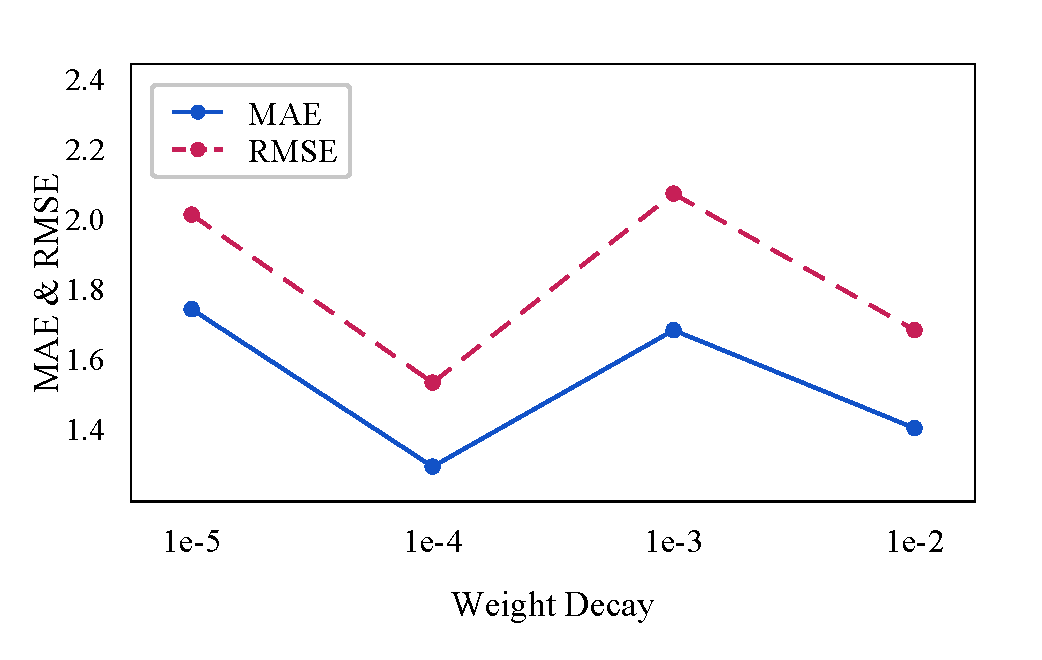
\includegraphics[height=0.31\linewidth]{decay.pdf}}
\caption{Sensitivity to (a) learning rate and (b) weight decay on Classroom. Each experiment varies one hyperparameter while fixing the other settings.}
\label{fig:hyperparameters}
\end{figure}

\section{Conclusion and Discussion}
This paper presented WaveLoop, a temporal-frequency wavelet modulation framework for video crowd counting. Instead of coupling adjacent-frame information into an undifferentiated temporal representation, WaveLoop decomposes it into temporally shared content and rapid inter-frame variations and uses these complementary cues to reconfigure the current-frame frequency representation. SAFF first calibrates spatial wavelet bands with different response magnitudes. TFRM then performs content-adaptive temporal-frequency modulation, while DGFA introduces density-conditioned spatial guidance to coordinate spatial and frequency-domain features. DSE further reinforces strongly agreed responses from the temporal-frequency and spatial-frequency pathways, and supervised density-variation learning constrains the predicted inter-frame changes to follow the annotated density evolution.

Experiments on five video crowd counting benchmarks show that WaveLoop consistently improves frame-level counting accuracy and achieves competitive or state-of-the-art MAE/RMSE results. The cumulative component study verifies that each stage of the proposed design contributes to the complete framework, while the loss-weight, kernel-size, transfer-learning, and complexity analyses clarify its behavior under different settings. In particular, the results support the benefit of jointly exploiting stable temporal content, motion-sensitive variations, and density-aware cross-domain coordination rather than relying solely on current-frame appearance.

WaveLoop still has several limitations. First, the current temporal decomposition is constructed from adjacent frames and therefore captures only short-range temporal context. Extending the framework to longer clips without substantially increasing memory and computation remains an open problem. Second, the fixed wavelet basis may be less adaptive to abrupt camera motion, severe illumination changes, and highly nonstationary crowd dynamics. Third, the additional temporal-frequency encoders and multi-scale cross-domain interaction increase latency relative to lighter video counting models. Future work will investigate adaptive temporal transforms, longer-range yet efficient temporal aggregation, and lightweight interaction mechanisms. Direct evaluation of density-variation fidelity and robustness under camera motion would also provide a more complete assessment of temporal behavior.

\bibliographystyle{IEEEtran} 
\bibliography{refs}



\begin{IEEEbiography}[{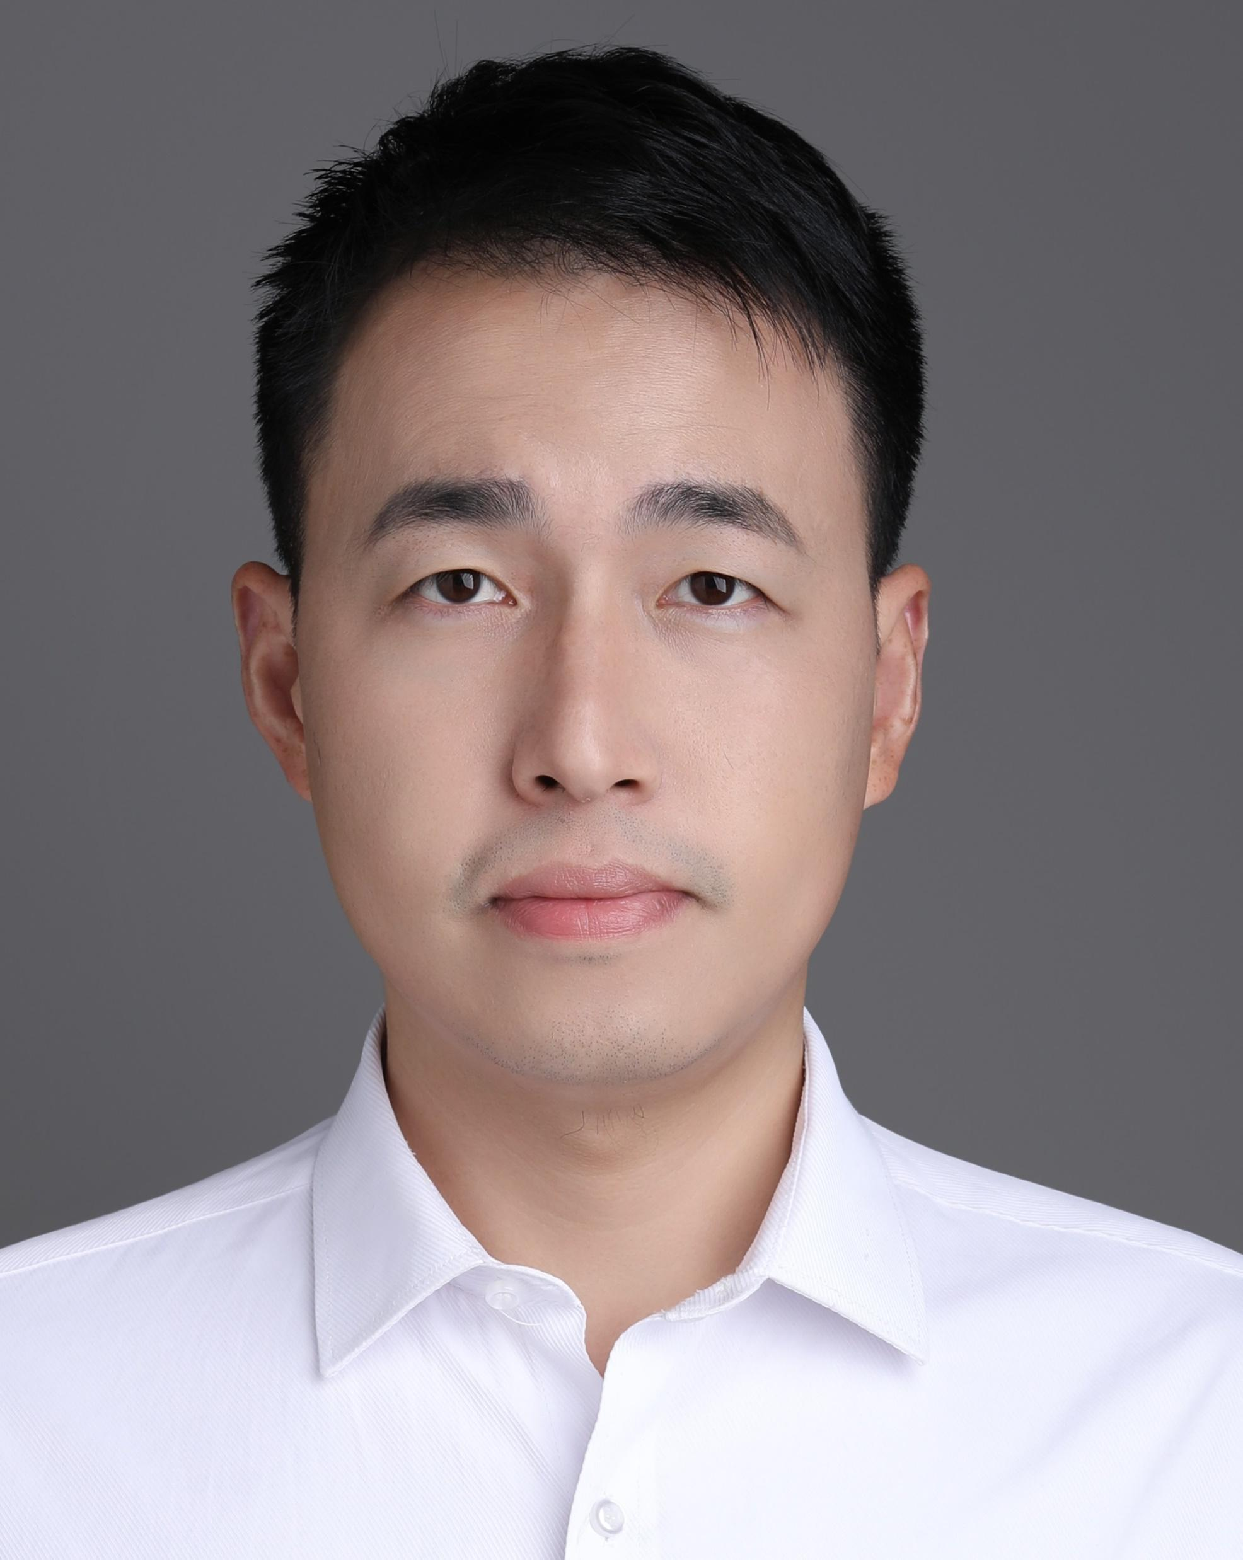
\includegraphics[width=1in,height=1.25in,clip,keepaspectratio]{ling.pdf}}]{Miaogen Ling} is currently an associate professor at Nanjing University of Information Science and Technology, China. He received the B.S. (2010) degree in mathematical science from the Soochow University, China and the M.S. degree and the Ph.D (2019) degree in computer science from the Southeast University, China. His research interests include deep learning and its application to computer vision and multimedia analysis.
\end{IEEEbiography}

\vspace{-3em}

\begin{IEEEbiography}
[{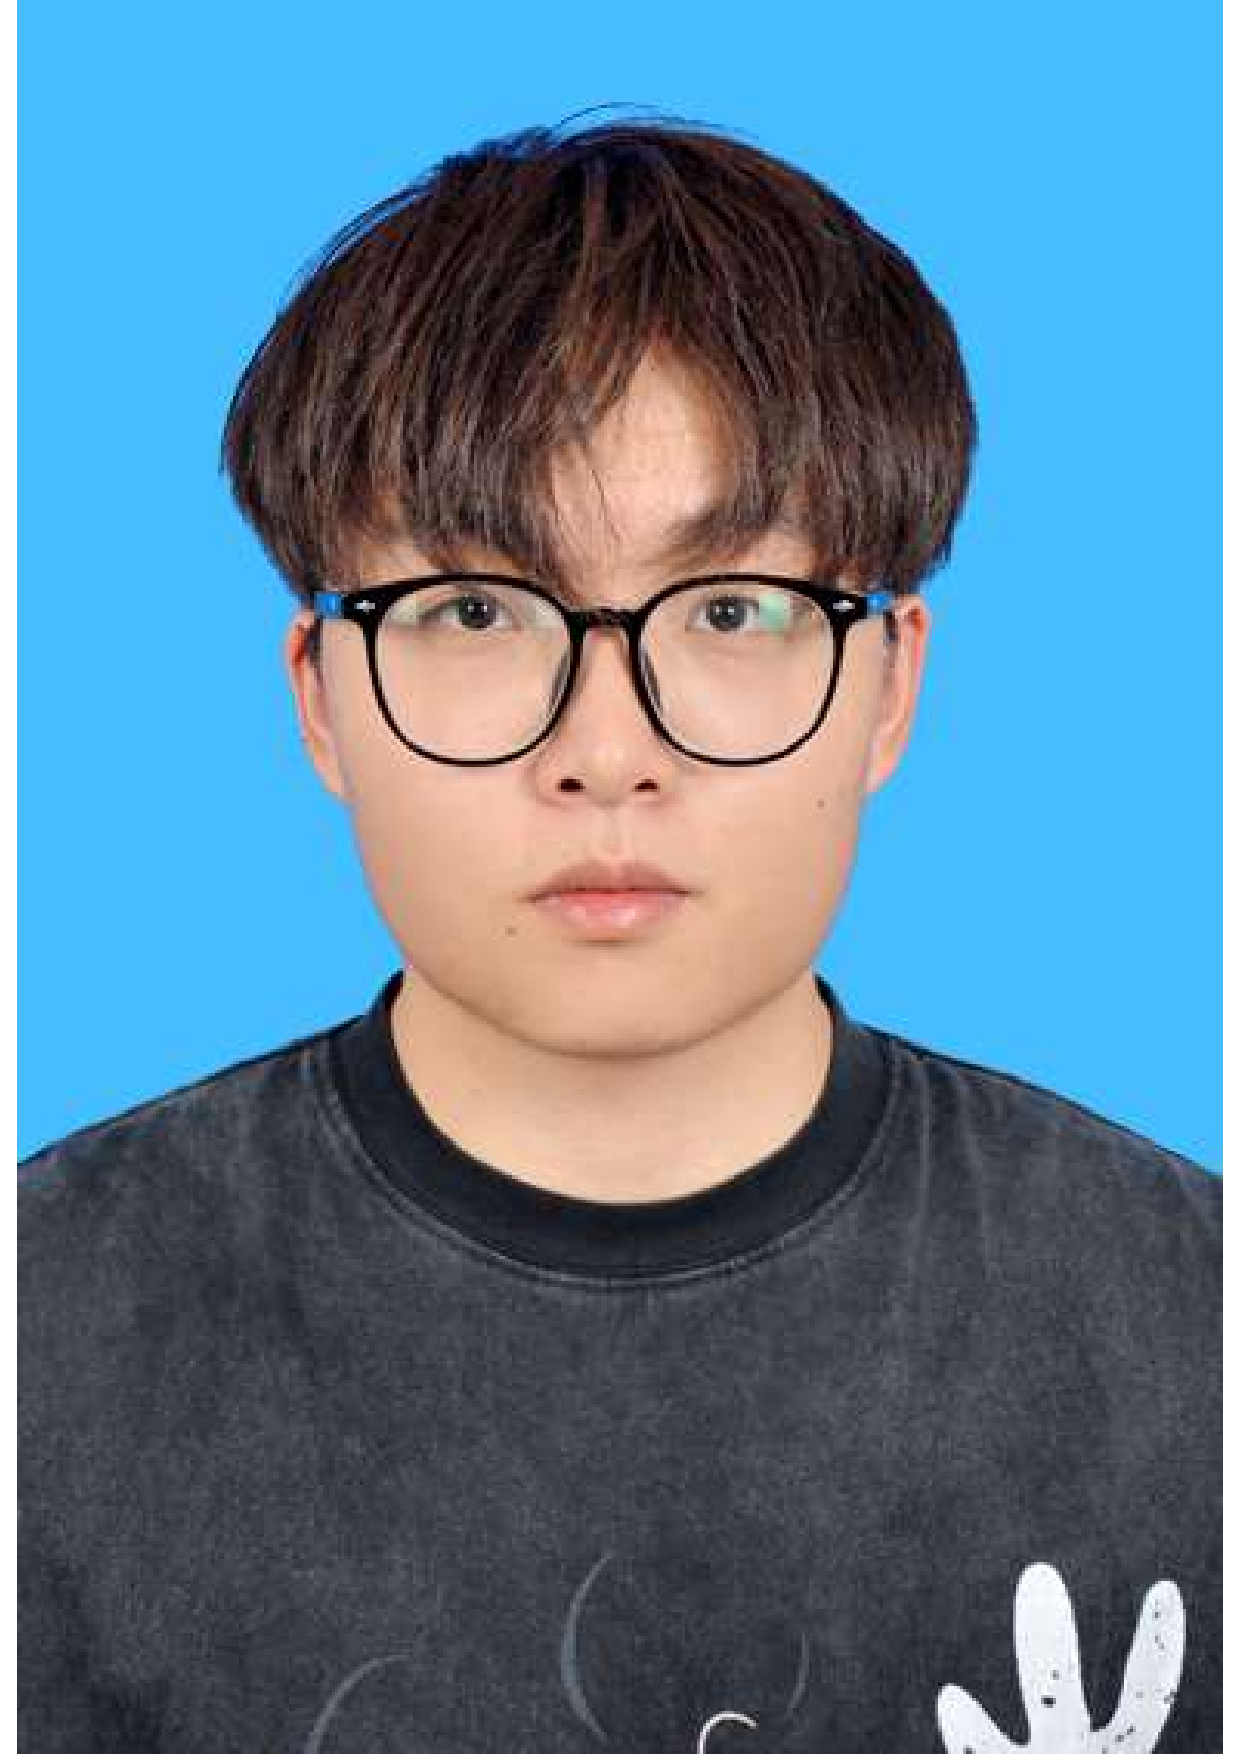
\includegraphics[width=1in,height=1.25in,clip]{sun.pdf}}]{Junyu Sun}
is currently pursuing the M.S. degree in Computer Science and Technology at Nanjing University of Information Science and Technology, China. He received the B.S. degree in Computer Science and Technology from SanJiang University, China, in 2024. His research interests include deep learning and its applications in computer vision.
\end{IEEEbiography}

\vspace{-3em}

\begin{IEEEbiography}
[{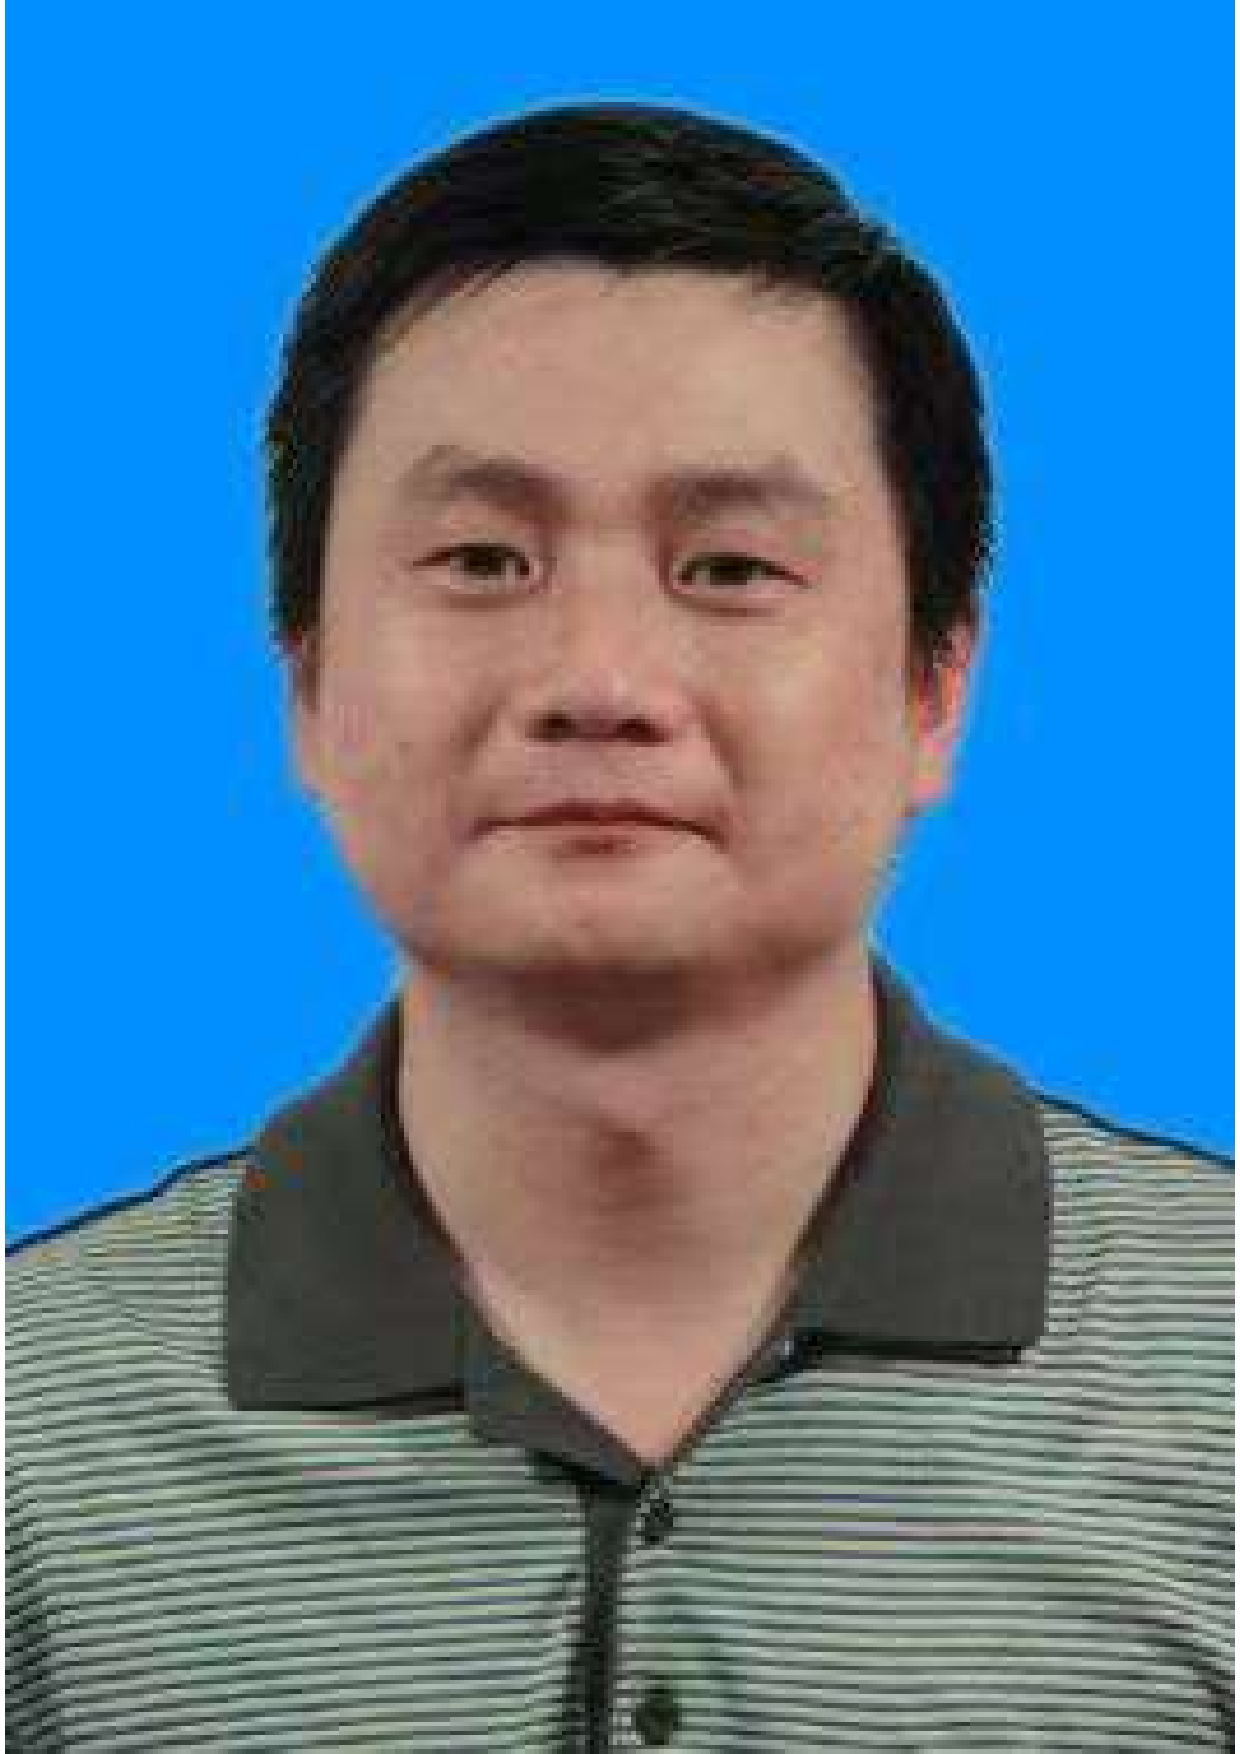
\includegraphics[width=1in,height=1.25in,clip]{fang.pdf}}]{Wei Fang} received the M.Sc. and Ph.D. degrees in computer science from Soochow University, Suzhou, China. He is currently a Professor with Jiangsu Engineering Center of Network Monitoring, Nanjing University of Information Science and Technology, Nanjing, China, State Key Laboratory for Novel Software Technology, Nanjing University, Nanjing. His research interests are in the areas of artificial
intelligence, big data analysis of meteorology, deep learning and cloud computing. Dr. Fang is a PC member for a number of international conferences and a reviewer for several international journals.
\end{IEEEbiography}

\vspace{-3em}

\begin{IEEEbiography}
[{
\includegraphics[width=1in,height=1.25in,clip,keepaspectratio]{geng.pdf}}]{Xin Geng} (Senior Member, IEEE) is a chair professor of Southeast University, China. His research interests include machine learning, pattern recognition, and computer vision. He has published over 100 refereed papers in these areas. He has been an Associate Editor of IEEE T-MM, FCS and MFC, a Steering Committee Member of PRICAI, a Program Committee Chair for conferences such as PRICAI’18, VALSE’13, etc., an Area Chair for conferences such as IJCAI, CVPR, ACMMM, ICPR, and a Senior Program Committee Member for conferences such as IJCAI, AAAI, ECAI, etc. He is a Distinguished Fellow of IETI and a Senior Member of IEEE.
\end{IEEEbiography}

\vfill

\end{document}


